\documentclass[11pt]{article}

\usepackage[utf8]{inputenc}
\usepackage[T1]{fontenc}
\usepackage[USenglish]{babel}
\usepackage[a4paper,margin=32mm,headheight=14pt]{geometry}
\usepackage{lmodern}
\usepackage{microtype}
\usepackage{csquotes}
\usepackage{amsmath,amssymb}
\usepackage{amsthm}
\usepackage{xcolor}
\usepackage{tikz}
\usepackage{fancyhdr}
\usepackage[
  colorlinks=true,
  linkcolor=blue!45!black,
  citecolor=green!35!black,
  urlcolor=blue!55!black,
  pdfauthor={Alex Junior Gomez Saltachin},
  pdftitle={Categorical genus for log del Pezzo surfaces with cyclic quotient singularities},
  pdfsubject={Algebraic geometry and mirror symmetry},
  pdfkeywords={Log del Pezzo surfaces, canonical stacks, cyclic quotient singularities, categorical mirror genus, maximally mutable Laurent polynomials}
]{hyperref}
\usepackage[capitalize,nameinlink]{cleveref}

\theoremstyle{plain}
\newtheorem{theorem}{Theorem}[section]
\newtheorem{proposition}[theorem]{Proposition}
\newtheorem{lemma}[theorem]{Lemma}
\newtheorem{corollary}[theorem]{Corollary}
\newtheorem*{citedtheorem}{Theorem}
\theoremstyle{definition}
\newtheorem{definition}[theorem]{Definition}
\newtheorem{example}[theorem]{Example}
\theoremstyle{remark}
\newtheorem{remark}[theorem]{Remark}

\crefname{theorem}{Theorem}{Theorems}
\crefname{proposition}{Proposition}{Propositions}
\crefname{lemma}{Lemma}{Lemmas}
\crefname{corollary}{Corollary}{Corollaries}
\crefname{definition}{Definition}{Definitions}
\crefname{example}{Example}{Examples}
\crefname{remark}{Remark}{Remarks}

\newcommand{\cX}{\mathcal X}
\newcommand{\Db}{\mathrm D^b}
\newcommand{\coh}{\operatorname{coh}}
\newcommand{\NS}{\operatorname{NS}}
\newcommand{\rk}{\operatorname{rk}}
\newcommand{\Span}{\operatorname{Span}}
\newcommand{\Ext}{\operatorname{Ext}}
\newcommand{\C}{\mathbb C}
\newcommand{\Q}{\mathbb Q}
\newcommand{\Z}{\mathbb Z}
\newcommand{\Pj}{\mathbb P}
\newcommand{\1}{\mathbf 1}

\usepackage[
  backend=biber,
  style=numeric-comp,
  sorting=nyt,
  sortcites=true,
  giveninits=true,
  doi=true,
  url=false,
  isbn=false
]{biblatex}
\addbibresource{bibliography.bib}

\pagestyle{fancy}
\fancyhf{}
\fancyhead[L]{\small A. J. Gomez Saltachin}
\fancyhead[R]{\small Categorical genus for cyclic quotient surfaces}
\fancyfoot[C]{\thepage}
\renewcommand{\headrulewidth}{0.4pt}
\renewcommand{\footrulewidth}{0pt}
\fancypagestyle{plain}{%
  \fancyhf{}
  \fancyfoot[C]{\thepage}
  \renewcommand{\headrulewidth}{0pt}
  \renewcommand{\footrulewidth}{0pt}}
\setlength{\parindent}{1.5em}
\setlength{\parskip}{0pt}
\emergencystretch=2em

\begin{document}

\title{Categorical genus for log del Pezzo surfaces with cyclic quotient singularities}
\author{Alex Junior Gomez Saltachin\\[0.5em]
\small Departamento de Matem\'atica, Pontif\'icia Universidade Cat\'olica do Rio de Janeiro\\
\small Rua Marqu\^es de S\~ao Vicente, 225, Rio de Janeiro, RJ 22451-900, Brazil\\
\small \href{mailto:alex.gomez@pucp.edu.pe}{alex.gomez@pucp.edu.pe}}
\date{}

\maketitle

\begin{abstract}
For the canonical stack $\cX$ of a log del Pezzo surface with cyclic quotient singularities, we compute its categorical genus as
\[
g_{\mathrm{cat}}(\cX)=1+\frac12\sum_j w_j(\ell_j-1),
\]
where $w_j=\gcd(n_j,q_j+1)$ and $\ell_j=n_j/w_j$ are the local widths and Gorenstein indices of the singularities $\frac1{n_j}(1,q_j)$.  Serre duality and inertial Riemann--Roch separate the smooth contribution from the local canonical characters, and identify categorical genus with $1+\dim H^{\operatorname{age}<1}_{\cX}$.  Passing to a sufficiently general $\Q$-Gorenstein deformation defines the residual invariant $g_{\mathrm{cat}}^{\mathrm{qG}}(X)$; its difference from $g_{\mathrm{cat}}(\cX)$ is exactly the weighted $T$-content contribution.  For any surface admitting a toric $\Q$-Gorenstein degeneration, this identifies the residual categorical invariant with Tveiten's mutable genus, the genus of a general maximally mutable Laurent-polynomial fiber for the chosen degeneration.  The locally $\Q$-Gorenstein rigid comparison is the special case in which the drop vanishes.  For toric surfaces, the categorical genus of the given canonical stack counts all interior lattice points and equals the genus of a general Laurent-polynomial fiber.  Explicit Oneto--Petracci mirrors give direct checks.
\end{abstract}

\medskip
\noindent\textbf{2020 Mathematics Subject Classification.}
Primary 14F08; Secondary 14J45, 14A20, 14M25.

\smallskip
\noindent\textbf{Keywords.}
Log del Pezzo surfaces, canonical stacks, cyclic quotient singularities, skew Euler form, maximally mutable Laurent polynomials.

\section{Introduction}

For a smooth del Pezzo surface $Y$, the antisymmetric part of the numerical Euler pairing has rank $2$, as follows from Hirzebruch--Riemann--Roch in Kuznetsov's numerical coordinates \cite[Example 3.5]{Kuz} (Corollary~\ref{ex:smooth-del-pezzo}).  On the mirror side, a general Landau--Ginzburg fiber has a smooth projective compactification of genus one \cite{galkin2008delpezzo,AKO}.  This agreement suggests that half the rank of the skew Euler form may behave like a genus.  What becomes of this relation when the surface acquires quotient singularities?

The motivating singular example is the general hypersurface $X_{10}\subset\Pj(1,2,3,5)$, which has a single $\frac13(1,1)$ point \cite[Section 7.3, entry 11]{OP}.  Its canonical smooth Deligne--Mumford stack $\cX_{10}$ has a skew Euler form of rank $4$, while its mirror curve has genus two.  The full exceptional collection in the author's earlier paper \cite[Proposition 5.4]{GS} gives this rank, in agreement with the intrinsic calculation in Example~\ref{ex:x10-rank}.  After reading that paper, Sergey Galkin suggested that half the rank of the antisymmetrized Euler matrix of an exceptional collection should reflect the genus of the mirror curve.  His suggestion motivates the present study.

The main contribution of this paper is the intrinsic cyclic basket formula of Theorem~\ref{thm:intro-cyclic}: the skew Euler rank, or equivalently its half-rank, is computed for arbitrary cyclic quotient singularities by the Serre operator and numerical inertial Riemann--Roch.  This proof requires neither a full exceptional collection, a toric degeneration, nor homological mirror symmetry.  We name the half-rank \emph{categorical genus}, interpret its local corrections through age, and establish its $\Q$-Gorenstein residual formula and exact categorical $T$-content drop.  The mirror-side contribution is the identification of this residual categorical genus with Tveiten's mutable genus.  Singularity content and residual cones \cite{AkhtarKasprzyk}, together with Tveiten's genus formula \cite[Theorem 3.13]{Tveiten}, are the known mirror-side inputs.  The special McKay calculation supplies a geometric model in the $\frac13(1,1)$ case.

Write $\chi^-:=\chi-\chi^{\mathsf T}$ for the skew Euler form.  We define the \emph{categorical genus} of a smooth proper surface stack $\mathcal X$ by
\[
g_{\mathrm{cat}}(\mathcal X)
:=\frac12\rk_{\Q}\chi^-_{\mathcal X}.
\]
The pairing is taken on $K_0^{\mathrm{num}}(\mathcal X)_{\Q}$.  An alternating form on a finite-dimensional vector space over a field of characteristic zero has even rank, so half its rank is an integer.  It is an invariant of the $\C$-linear triangulated category $\Db(\coh\mathcal X)$: an exact equivalence preserves the Euler pairing and its numerical quotient.  A full exceptional collection provides a matrix representation (Definition~\ref{def:categorical-genus}).

Homological mirror symmetry motivates the relation between skew Euler rank and mirror-fiber genus.  Harder--Thompson's pseudolattice description of genus-one Lefschetz fibrations compares numerical $K$-theory with its Euler pairing to relative homology with its Seifert pairing \cite[Sections 4.2 and 5]{HarderThompson}.  The antisymmetrization of the latter is, up to sign, the pullback of the fiber intersection form under the boundary map.  When vanishing cycles span the nondegenerate genus part of fiber homology, this suggests skew rank $2g$ for a genus-$g$ fiber.

Simeonov's 2026 preprint, in its second version, proves homological mirror symmetry for effective orbifold log Calabi--Yau surfaces at the large complex structure limit \cite[Definition 1.1 and Theorem 0.1]{Simeonov}.  These are rational projective orbifold surfaces with isolated cyclic quotient singularities and an effective nodal anticanonical stacky cycle whose nodes contain the orbifold points; the minimal resolution is required to have the distinguished complex structure.  His theorem identifies the derived category of coherent sheaves with the derived Fukaya--Seidel category of a constructed exact Lefschetz fibration.  This setting allows general cyclic quotient types.  His theorem gives a categorical equivalence for surfaces satisfying these hypotheses, while our numerical formula applies to all cyclic quotient log del Pezzo surfaces.

The first evidence beyond $X_{10}$ comes from log del Pezzo surfaces $Z_k$ with $k$ singular points, all of type $\frac13(1,1)$, as in the Corti--Heuberger families \cite{CH}.  For their canonical stacks $\mathcal Z_k$, the special McKay decomposition of Ishii--Ueda \cite{IU} and the local adjoint calculation of Gugiatti--Rota \cite[Example 3.5]{GR} give
\[
\rk_{\Q}\chi^-_{\mathcal Z_k}=2k+2,
\qquad
g_{\mathrm{cat}}(\mathcal Z_k)=k+1.
\]
Proposition~\ref{prop:third-rank} gives a contribution of $2$ to the rank of the skew Euler form from each singular point.

The weighted-projective stack $\mathcal P_n=\Pj(1,1,n)$, for $n\ge2$, provides the model calculation that reveals how this correction varies.  Its coarse space has one point of type $\frac1n(1,1)$, and the Serre-operator computation in Proposition~\ref{prop:weighted-rank} gives
\[
\rk_{\Q}\chi^-_{\mathcal P_n}=2+n-\gcd(n,2),
\qquad
g_{\mathrm{cat}}(\mathcal P_n)=\left\lfloor\frac{n+1}{2}\right\rfloor.
\]
The rank is the untwisted contribution $2$ of the smooth case plus the local contribution $n-\gcd(n,2)$, recovering the preceding calculation at $n=3$.  What is the corresponding contribution of a cyclic quotient point $\frac1n(1,q)$?

\begin{theorem}[Categorical genus for cyclic quotient surfaces; Theorem~\ref{thm:cyclic-rank}]\label{thm:intro-cyclic}
Let $X$ be a log del Pezzo surface whose singularities are of type $\frac1{n_j}(1,q_j)$, $j=1,\dots,s$, and let $\cX$ be its canonical smooth Deligne--Mumford stack.  Write $w_j=\gcd(n_j,q_j+1)$ for the width and $\ell_j=n_j/w_j$ for the local Gorenstein index.  The rank of its skew Euler form is
\[
\rk_{\Q}\chi^-_{\cX}
=2+\sum_{j=1}^s\bigl(n_j-\gcd(n_j,q_j+1)\bigr),
\]
and hence
\[
g_{\mathrm{cat}}(\cX)
=1+\frac12\sum_{j=1}^s w_j(\ell_j-1).
\]
\end{theorem}

The local rule is $(n-\gcd(n,q+1))/2=w(\ell-1)/2$ per singular point, in addition to the global contribution one.  It is useful to distinguish three invariants from the outset.  Write $w=m\ell+w_0$, $0\le w_0<\ell$; intuitively, $w_0$ is the width left after all locally smoothable content has been removed.  With the precise terminology deferred to Section~\ref{sec:mirror}, the table anticipates the residual formula and mirror comparison of Theorem~\ref{thm:intro-mirror}:
\begin{center}
\renewcommand{\arraystretch}{1.25}
\begin{tabular}{@{}lll@{}}
\hline
Invariant & What it records & Value\\\hline
$g_{\mathrm{cat}}(\cX)$ & the given canonical stack
& $1+\frac12\sum_j w_j(\ell_j-1)$\\
$g_{\mathrm{cat}}^{\mathrm{qG}}(X)$ & a general $\Q$-Gorenstein deformation
& $1+\frac12\sum_j w_{0,j}(\ell_j-1)$\\
$g_{\mathrm{MMLP}}$ & a general mirror fiber
& $g_{\mathrm{cat}}^{\mathrm{qG}}(X)$\textsuperscript{$\ast$}\\\hline
\end{tabular}
\end{center}
\noindent\textsuperscript{$\ast$}For a surface admitting a toric $\Q$-Gorenstein degeneration with polygon $P$, the last equality holds for a general maximally mutable Laurent polynomial with Newton polygon $P$, as in Theorem~\ref{thm:intro-mirror}.  Here $R$ denotes the residual lattice-point set of the polygon.  For a toric surface $X_P$, the first row is $\#(P^\circ\cap N)$ and the other two are $1+\#(R\cap P^\circ)$; the all-interior-point interpretation is specifically toric.  Cyclic Du Val points contribute zero.  Non-Du Val $T$-singularities contribute to the given stack but disappear from its categorical genus under general $\Q$-Gorenstein deformation.  Theorem~\ref{thm:intro-mirror} quantifies this loss and identifies the residual value with mirror genus, whether or not $X$ is locally $\Q$-Gorenstein rigid.

The formula separates the untwisted rank-$2$ contribution, already present for every smooth del Pezzo surface by Corollary~\ref{ex:smooth-del-pezzo}, from the local cyclic corrections.  In the proof of Theorem~\ref{thm:cyclic-rank}, Serre duality identifies the rank of the skew Euler form with $\rk(1-S)$, where $S$ is the Serre operator, and inertial Riemann--Roch separates the untwisted and twisted sectors.  At $\frac1n(1,q)$, the canonical character on the sector indexed by $i$ has eigenvalue $\zeta^{-i(q+1)}$, for a primitive $n$th root $\zeta$; counting the fixed sectors produces $\gcd(n,q+1)$.

This local formula admits a second interpretation in terms of age.  Write
\[
H^{\operatorname{age}<1}_{\cX}
:=\bigoplus_{0<\operatorname{age}(\gamma)<1}\C\1_\gamma
\]
for the space with one basis vector for each nontrivial twisted sector $\gamma$ of the inertia stack $I\cX$ of age less than one.

\begin{theorem}[The age interpretation; Theorem~\ref{thm:age-interpretation}]\label{thm:intro-age}
For the canonical stack $\cX$ of a log del Pezzo surface with cyclic quotient singularities,
\[
g_{\mathrm{cat}}(\cX)=1+\dim H^{\operatorname{age}<1}_{\cX}.
\]
\end{theorem}

Pairing the sectors indexed by $i$ and $n-i$ gives the local age count (Lemma~\ref{lem:age-count}), from which Theorem~\ref{thm:age-interpretation} derives the global identity.  This is a reformulation of the categorical formula, whose proof does not use age.

For a fixed Newton polygon $P$, we denote Tveiten's \emph{mutable genus} by
\[
g_{\mathrm{MMLP}}:=g_{\mathrm{mut}}(P)=1+\#(R\cap P^\circ).
\]
Tveiten proves that this is the genus of the smooth projective model of a generic maximally mutable Laurent-polynomial fiber and is invariant under mutation \cite[Theorem 3.13]{Tveiten}.  We use the formulation of this genus theorem in \cite[Theorem 3.13]{CKPT}.

To identify this mirror invariant categorically for surfaces admitting toric $\Q$-Gorenstein degenerations, one must first remove the smoothable local content.  Precise definitions are collected in Section~\ref{sec:mirror}.  Section~\ref{sec:qg-generic} computes the categorical genus of a sufficiently general deformation and its exact difference from the original genus.  The local lattice count in Lemma~\ref{lem:age-count} then identifies the surviving categorical contribution with mutable genus.

For a log del Pezzo surface $X$ with cyclic quotient singularities, let $\mathcal X_t$ be the canonical stack of a sufficiently general fiber of a miniversal $\Q$-Gorenstein deformation.  Set
\[
g_{\mathrm{cat}}^{\mathrm{qG}}(X):=g_{\mathrm{cat}}(\mathcal X_t).
\]
This residual categorical genus is defined formally in Definition~\ref{def:qg-generic-genus}; independence of the choices is part of the following theorem.

\begin{theorem}[Categorical genus under deformation and mirror genus]\label{thm:intro-mirror}
Let $X$ be a log del Pezzo surface with cyclic quotient singularities and canonical stack $\cX$.  At each singular point, use the widths and indices of Theorem~\ref{thm:intro-cyclic} and write
\[
w_j=m_j\ell_j+w_{0,j},\qquad 0\le w_{0,j}<\ell_j.
\]
The value $g_{\mathrm{cat}}^{\mathrm{qG}}(X)$ is independent of the sufficiently general fiber and the chosen miniversal deformation, and satisfies
\[
\begin{aligned}
g_{\mathrm{cat}}^{\mathrm{qG}}(X)
&=1+\frac12\sum_j w_{0,j}(\ell_j-1),\\
g_{\mathrm{cat}}(\cX)-g_{\mathrm{cat}}^{\mathrm{qG}}(X)
&=\sum_j m_j\binom{\ell_j}{2}.
\end{aligned}
\]
If moreover $X$ admits a toric $\Q$-Gorenstein degeneration, choose one to $X_{P_0}$, and let $P$ be $P_0$ or a mutation-equivalent Fano polygon with the same residual basket.  For a general maximally mutable Laurent polynomial $f$ with Newton polygon $P$ and a general value $\eta$,
\[
g_{\mathrm{cat}}^{\mathrm{qG}}(X)
=1+\#(R\cap P^\circ)
=g\bigl(\widetilde{\{f=\eta\}}\bigr),
\]
where $R$ is the residual set of $P$ and the tilde denotes the smooth projective model of the fiber.
\end{theorem}

The mirror assertion of Theorem~\ref{thm:intro-mirror} is therefore the new identification with Tveiten's existing invariant,
\[
\boxed{g_{\mathrm{cat}}^{\mathrm{qG}}(X)=g_{\mathrm{MMLP}}.}
\]
The theorem combines Lemma~\ref{lem:generic-residual-basket}, Proposition~\ref{prop:qg-residual-genus}, and Corollaries~\ref{cor:t-content-drop} and~\ref{cor:qg-generic-mirror-genus}.  Neither the residual formula nor the drop formula requires a toric $\Q$-Gorenstein degeneration; that hypothesis enters only in the mirror comparison.  Under its boundary nondegeneracy hypotheses, Proposition~\ref{prop:boundary-delta} identifies the categorical $T$-content drop with the boundary genus defect already described by Tveiten \cite[Remark 3.14, arXiv version 2]{Tveiten}.  The genus is independent of the chosen toric degeneration, without assuming that two such polygons are mutation equivalent; see the discussion following Corollary~\ref{cor:qg-generic-mirror-genus}.  The locally rigid comparison is an immediate special case.

\begin{corollary}[The locally $\Q$-Gorenstein rigid case]\label{cor:intro-rigid}
With the notation and choices of Theorem~\ref{thm:intro-mirror}, if $X$ is locally $\Q$-Gorenstein rigid and admits a toric $\Q$-Gorenstein degeneration, then
\[
g_{\mathrm{cat}}(\cX)
=g_{\mathrm{cat}}^{\mathrm{qG}}(X)
=g\bigl(\widetilde{\{f=\eta\}}\bigr).
\]
\end{corollary}

Indeed, local rigidity means $m_j=0$ at every singular point, so the $T$-content drop vanishes.  Section~\ref{sec:mirror} also proves this case directly in Theorem~\ref{cor:genus-match}.

\begin{corollary}[The toric case]\label{cor:intro-toric}
Let $P\subset N_{\mathbb R}$ be a Fano polygon and let $\mathcal X_P$ be the canonical stack of the toric del Pezzo surface defined by the fan over the faces of $P$.  Then
\[
g_{\mathrm{cat}}(\mathcal X_P)=\#(P^\circ\cap N).
\]
Consequently, for a general Laurent polynomial $h$ with Newton polygon $P$ and a general value $\eta$,
\[
g_{\mathrm{cat}}(\mathcal X_P)=g\bigl(\widetilde{\{h=\eta\}}\bigr).
\]
\end{corollary}

This is Proposition~\ref{prop:toric-categorical-genus} together with Corollary~\ref{cor:toric-laurent-genus}.  A general Laurent polynomial records all interior points, whereas a general maximally mutable Laurent polynomial records only the residual points and the origin.  Thus the hierarchy runs from the categorical genus of the given stack, through its age interpretation, to the $\Q$-Gorenstein generic residual genus and then to mirror genus.

The surface $X=\Pj(1,1,4)$ shows why passing to a general $\Q$-Gorenstein deformation is necessary even for toric surfaces.  Its canonical stack has categorical genus two, but its $\frac14(1,1)$ point is a smoothable $T$-singularity, so $g_{\mathrm{cat}}^{\mathrm{qG}}(X)=1$, the genus of a general maximally mutable Laurent polynomial fiber.  The extra contribution belongs to the given stack and disappears under a sufficiently general $\Q$-Gorenstein deformation.  Local rigidity eliminates this distinction.

For the Corti--Heuberger surfaces, the categorical formula gives $g_{\mathrm{cat}}=k+1$ throughout all $29$ deformation families \cite{CH}.  Their $\frac13(1,1)$ points are locally $\Q$-Gorenstein rigid, and exactly $26$ families admit toric $\Q$-Gorenstein degenerations \cite[Theorem 8]{ACC+}; on these, $k+1$ is the genus of a general maximally mutable Laurent polynomial fiber.  In particular, the case of $X_{10}$ recovers the motivating genus-two prediction.

There is concrete mirror evidence beyond this genus-two case.  Oneto--Petracci \cite[Theorem 2.2]{OP} compare classical periods of explicit maximally mutable Laurent polynomials with restrictions of quantum periods for del Pezzo surfaces with $\frac13(1,1)$ points admitting toric $\Q$-Gorenstein degenerations.  Their result is conditional on the orbifold Quantum Lefschetz and Abelian/non-Abelian conjectures stated in \cite[Conjectures 5.2 and 6.1]{OP}.  Their polynomials predate categorical genus and provide independent models on which to test its numerical meaning.  Representative mirror families with $k=1,2,3,4,6$ give genera $2,3,4,5,7$, respectively, agreeing with $g_{\mathrm{cat}}=k+1$.  These direct checks complement the general maximally mutable Laurent polynomial genus theorem; the six-point case also illustrates why the Newton polygon and generality matter.  Petracci's toric example \cite{PetracciKmoduli} distinguishes the genus of the actual stack from that of a generic $\Q$-Gorenstein deformation.  Section~\ref{sec:qg-generic} measures this difference exactly by the $T$-content and identifies the toric categorical genus with the full interior-lattice-point count.

Section~\ref{sec:categorical} introduces categorical genus through the smooth case and the special McKay calculation for $\frac13(1,1)$ singularities.  Section~\ref{sec:serre} develops the intrinsic Serre-operator method and proves the cyclic quotient formula.  Section~\ref{sec:age} identifies the local corrections with age and lattice-point counts.  Section~\ref{sec:mirror} introduces residual singularities and proves the locally rigid mirror comparison.  Section~\ref{sec:qg-generic} completes Theorem~\ref{thm:intro-mirror} by proving the residual formula, the exact $T$-content drop, and the general mirror comparison; it then interprets the drop through boundary singularities.  Section~\ref{sec:explicit-mirrors} collects the explicit mirror curves, deformation examples, and the scope of the comparison.  Appendix~\ref{app:numerical-inertia} supplies the numerical inertial Riemann--Roch argument.

\section{Categorical genus and the geometric model}\label{sec:categorical}

We begin with the Euler pairing on a smooth surface and use its antisymmetric part to define categorical genus.  The special McKay correspondence then gives a geometric calculation for $\frac13(1,1)$ singularities.

We work over $\C$; all stacks considered are separated Deligne--Mumford stacks of finite type, hence tame.  The geometric setting is the same as in the author's earlier study of exceptional collections on canonical stacks of log del Pezzo surfaces with $\frac13(1,1)$ singularities \cite{GS}.

\begin{definition}[Log del Pezzo surfaces and canonical stacks]
A log del Pezzo surface is a normal projective surface $X$ with quotient singularities and ample $-K_X$.  Its basket of singularities is the multiset of its singularity types, counted with multiplicity.  Its canonical stack $\cX$ is the smooth Deligne--Mumford stack with coarse space $X$ and no stabilizers away from the singular points.
\end{definition}


\begin{definition}[Euler pairing and numerical Grothendieck group]
For a smooth proper Deligne--Mumford stack $\mathcal Z$, the Euler pairing and its antisymmetric part are
\[
\chi_{\mathcal Z}(E,F)
=\sum_i(-1)^i\dim\Ext^i(E,F),
\qquad
\chi_{\mathcal Z}^-(E,F)
:=\chi_{\mathcal Z}(E,F)-\chi_{\mathcal Z}(F,E).
\]
We use $K_0^{\mathrm{num}}(\mathcal Z)=K_0(\mathcal Z)/\operatorname{rad}\chi_{\mathcal Z}$.
\end{definition}

The left and right radicals agree: Serre duality gives $\chi(v,u)=\chi(u,Sv)$, where $S$ is the automorphism induced by the Serre functor.  Thus vanishing against every class in either argument is equivalent to vanishing in the other.

Unless another coefficient field is indicated, all Grothendieck groups in this section are tensored with $\Q$.  For a smooth projective surface $Y$, Kuznetsov \cite[Example 3.5]{Kuz} describes the numerical group as
\[
K_0^{\mathrm{num}}(Y)_{\Q}
\simeq
\Q\oplus\NS(Y)_{\Q}\oplus\Q,
\]
with coordinates represented by rank, first Chern class, and a degree-two class.  Hirzebruch--Riemann--Roch shows that only the first two coordinates enter the skew form.

\begin{lemma}[The smooth-surface skew form]\label{lem:RR-skew}
For $A,B\in K_0(Y)_{\Q}$, write $r_A=\rk(A)$ and $D_A=c_1(A)$, with analogous notation for $B$.  Their skew Euler pairing is
\begin{equation}\label{eq:smooth-skew}
\chi_Y^-(A,B)
=-K_Y\cdot\bigl(r_A D_B-r_BD_A\bigr).
\end{equation}
\end{lemma}

\begin{proof}
Hirzebruch--Riemann--Roch gives
\[
\chi_Y(A,B)=\int_Y
\operatorname{ch}(A^\vee)\operatorname{ch}(B)\operatorname{td}(Y).
\]
The degree-two part of $\operatorname{ch}(A^\vee)\operatorname{ch}(B)$ is the symmetric expression
\[
r_A\operatorname{ch}_2(B)+r_B\operatorname{ch}_2(A)-D_A D_B.
\]
The contribution involving $\operatorname{td}_2(Y)$ is also symmetric, so both cancel upon antisymmetrization.  The remaining term comes from $\operatorname{td}_1(Y)=-K_Y/2$.  Since the degree-one component of
\[
\operatorname{ch}(A^\vee)\operatorname{ch}(B)
-\operatorname{ch}(B^\vee)\operatorname{ch}(A)
\]
is $2(r_A D_B-r_BD_A)$, integration gives \eqref{eq:smooth-skew}.
\end{proof}

\begin{corollary}[The smooth del Pezzo rank]\label{ex:smooth-del-pezzo}
Every smooth del Pezzo surface $Y$ satisfies
\begin{equation}\label{eq:smooth-rank-two}
\rk_{\Q}\chi_Y^-=2.
\end{equation}
\end{corollary}

\begin{proof}
In the rational coordinates $(r,D,c)=(\rk,c_1,\deg\operatorname{ch}_2)$, Lemma~\ref{lem:RR-skew} gives
\[
\chi_Y^-\bigl((r,D,c),(r',D',c')\bigr)
=-K_Y\cdot(rD'-r'D).
\]
Thus the degree-two coordinate lies in the radical, and the form has rank at most two because it depends only on the two linear functionals $r$ and $K_Y\cdot D$.  On the span of $e_0=(1,0,0)$ and $e_K=(0,K_Y,0)$ its matrix is
\[
\begin{pmatrix}0&-K_Y^2\\K_Y^2&0\end{pmatrix}.
\]
Since $K_Y^2>0$, this restriction is nondegenerate and the upper bound is attained.
\end{proof}

\begin{definition}[Categorical genus]\label{def:categorical-genus}
For a smooth proper surface stack $\cX$, its \emph{categorical genus} is
\[
\boxed{
g_{\mathrm{cat}}(\cX)
:=\frac12\rk_{\Q}\chi^-_{\cX},}
\]
where the pairing is taken on $K_0^{\mathrm{num}}(\cX)_{\Q}$.  The skew form factors through this numerical quotient, so the rank agrees with that computed on $K_0(\cX)_{\Q}$.
\end{definition}

The rank of the skew Euler form is even, so the definition is integral, and Corollary~\ref{ex:smooth-del-pezzo} gives $g_{\mathrm{cat}}(Y)=1$.  In the log del Pezzo setting, $g_{\mathrm{cat}}-1$ counts the additional two-dimensional nondegenerate summands of the skew form beyond this smooth rank-two contribution.

\begin{remark}[Choice of stack]\label{rem:choice-of-stack}
Categorical genus is an invariant of the chosen stack and its derived category, not of its coarse space alone.  Throughout the basket formulas we use the canonical stack.  Adding root-stack structure can change the inertia and the Euler pairing, so these formulas do not automatically apply to other stacks with the same coarse space.  Nor do we apply Definition~\ref{def:categorical-genus} to the singular coarse surface.  In Section~\ref{sec:qg-generic}, the $\Q$-Gorenstein generic invariant uses the canonical stack of a general deformed surface; it need not equal the invariant of the original canonical stack.
\end{remark}

We next compute the contribution of $\frac13(1,1)$ singularities by the special McKay correspondence.  This provides an independent proof in a special case and connects the invariant with exceptional collections: Proposition~\ref{prop:rank-span} expresses the rank through intersection pairings, and Proposition~\ref{prop:third-rank} evaluates it.  Readers interested only in the general formula may pass directly to the weighted-projective calculation in Proposition~\ref{prop:weighted-rank}.

For this calculation, let $X$ be a log del Pezzo surface with singular points $p_1,\dots,p_r$, all of this type.  Write $f:Y\to X$ for the minimal resolution and $C_i\subset Y$ for the exceptional curve over $p_i$.  The exceptional curves satisfy
\[
C_i\cdot C_j=-3\delta_{ij},
\]
and the canonical classes are related by the discrepancy formula
\begin{equation}\label{eq:discrepancy}
K_Y=f^*K_X-\frac13\sum_{i=1}^r C_i.
\end{equation}
The global cyclic case of the special McKay correspondence \cite[Proposition 8.1]{IU} gives a fully faithful functor $\Phi:\Db(\coh Y)\to\Db(\coh\cX)$ and a semiorthogonal decomposition
\begin{equation}\label{eq:IU-sod}
\Db(\coh\cX)
=\left\langle E_1,\dots,E_r,\Phi\Db(\coh Y)\right\rangle,
\end{equation}
Here $\Phi$ is the integral functor with kernel $\mathcal O_{(Y\times_X\cX)_{\mathrm{red}}}$.  The special McKay correspondence embeds the resolution category into the stack category; the remaining objects are supported at the singular points.

The \emph{special representations} are the trivial representation and those associated with exceptional curves on the minimal resolution; the others are called non-special \cite[Section 2.3]{GR}.

In \eqref{eq:IU-sod}, the exceptional object $E_i$ is the sheaf $(\iota_i)_*\rho_2$ supported on the residual gerbe $\iota_i:\mathcal B\mu_3\hookrightarrow\cX$, with the character convention specified below.  Objects at distinct points are orthogonal because their supports are disjoint, and the order in \eqref{eq:IU-sod} gives $R\!\operatorname{Hom}(\Phi A,E_i)=0$.

\begin{remark}[Character conventions]\label{rem:character-conventions}
In \cite[Section 2.3 and Example 2.7]{GR}, a generator $h$ has cotangent weights $(\zeta,\zeta)$ and $\rho_b(h)=\zeta^b$.  The special representations are $\rho_0,\rho_1$, so the complement uses $\rho_2$.  For the generator $g=h^{-1}$ acting on tangent vectors with weights $(\zeta,\zeta)$, $\rho_2(g)=\zeta^{-2}=\zeta$.  This specifies the sheaf, not just its support, and fixes the adjoint calculation below.
\end{remark}

For the left adjoint $\Psi$ of $\Phi$, the local calculation of Gugiatti--Rota \cite[Example 3.5]{GR}, specialized to $n=3$ and representation index $2$, gives
\[
\Psi(E_i)\simeq\mathcal O_{C_i}(-2).
\]
\begin{lemma}[Euler pairings with residual-gerbe sheaves]\label{lem:local-pairing}
For every $A\in K_0(Y)_{\Q}$, one has
\begin{equation}\label{eq:local-pairing}
\chi_{\cX}(E_i,\Phi A)=-c_1(A)\cdot C_i,
\qquad
\chi_{\cX}(\Phi A,E_i)=0.
\end{equation}
\end{lemma}

\begin{proof}
Semiorthogonality in \eqref{eq:IU-sod} gives the second equality.  For the first, adjunction yields
\[
\chi_{\cX}(E_i,\Phi A)=\chi_Y(\mathcal O_{C_i}(-2),A).
\]
Since locally free sheaves generate $K_0(Y)$, it suffices by additivity to take $A$ to be a vector bundle.  For the Cartier-divisor inclusion $j:C_i\hookrightarrow Y$, applying $R\mathcal{H}om_Y(-,A)$ to the Cartier divisor triangle
\[
\mathcal O_Y(-C_i)\longrightarrow\mathcal O_Y\longrightarrow j_*\mathcal O_{C_i}
\]
gives
\[
R\mathcal{H}om_Y(j_*\mathcal O_{C_i},A)
\simeq j_*\bigl(A|_{C_i}\otimes\mathcal O_{C_i}(C_i)\bigr)[-1].
\]
By the defining adjunction for $j^!$, this identifies
\[
j^!A=A|_{C_i}\otimes\mathcal O_{C_i}(C_i)[-1]
=A|_{C_i}\otimes\mathcal O_{C_i}(-3)[-1].
\]
Taking $R\!\operatorname{Hom}_{C_i}(\mathcal O_{C_i}(-2),j^!A)$ therefore gives
\[
R\!\operatorname{Hom}_Y(\mathcal O_{C_i}(-2),A)
\simeq
R\Gamma\bigl(C_i,A|_{C_i}\otimes\mathcal O_{C_i}(-1)\bigr)[-1],
\]
If $\delta_A=c_1(A)\cdot C_i$ is the degree of $A|_{C_i}$, Riemann--Roch on $C_i\simeq\Pj^1$ gives
\[
\chi\bigl(C_i,A|_{C_i}(-1)\bigr)=\delta_A.
\]
The shift $[-1]$ changes the sign of the Euler characteristic, proving \eqref{eq:local-pairing}.
\end{proof}

The smooth and local pairing formulas can now be assembled into a block matrix.  The minimal resolution $Y$ is rational: quotient singularities are rational, Kawamata--Viehweg vanishing gives $H^1(Y,\mathcal O_Y)=H^1(X,\mathcal O_X)=0$, and $-K_Y$ is big, so $H^0(Y,2K_Y)=0$.  Castelnuovo's criterion applies, as explained in \cite[Remark 4.3]{GR}.  We use a rational version of Kuznetsov's coordinates \cite[Example 3.5]{Kuz}, replacing the normalized Euler-characteristic coordinate by $\deg\operatorname{ch}_2$.  Explicitly, set
\[
\kappa:K_0(Y)_{\Q}\longrightarrow
\Q\oplus\NS(Y)_{\Q}\oplus\Q,
\qquad
[A]\longmapsto
\bigl(\rk(A),c_1(A),\deg\operatorname{ch}_2(A)\bigr).
\]
The rational Chern-character isomorphism described by Fulton \cite[Chapter 15]{Fulton} gives
\[
\operatorname{ch}_{\Q}:K_0(Y)_{\Q}\xrightarrow{\sim}
\operatorname{CH}^*(Y)_{\Q},
\]
and, since $Y$ is rational,
\[
\operatorname{CH}^0(Y)_{\Q}\cong\Q,
\qquad
\operatorname{CH}^1(Y)_{\Q}\cong\NS(Y)_{\Q},
\qquad
\operatorname{CH}^2(Y)_{\Q}\cong\Q.
\]
Thus $\kappa$ is an isomorphism.  Lemma~\ref{lem:RR-skew} shows that its third coordinate lies in the radical of the smooth skew form, while Lemma~\ref{lem:local-pairing} shows that it contributes nothing to the cross-pairings.

The semiorthogonal decomposition \eqref{eq:IU-sod} induces
\[
K_0(\cX)_{\Q}
\simeq
\bigoplus_{i=1}^r\Q[E_i]\oplus K_0(Y)_{\Q}.
\]
Using this decomposition and the coordinates $\kappa$, define
\[
e_0:=\Phi_*\bigl(\kappa^{-1}(1,0,0)\bigr),
\qquad
e_i:=[E_i]\quad(1\le i\le r).
\]
The rank and residual-gerbe classes span the subspace
\[
U:=\Q e_0\oplus\Q[E_1]\oplus\cdots\oplus\Q[E_r]
\subset K_0(\cX)_{\Q}.
\]
The rank of the skew Euler form can therefore be computed on $U\oplus\NS(Y)_{\Q}$, with the degree-two radical omitted.

\begin{proposition}[Rank from intersection pairings]\label{prop:rank-span}
The skew Euler form satisfies
\[
\rk_{\Q}\chi^-_{\cX}
=2\dim_{\Q}\Span\{K_Y,C_1,\dots,C_r\}.
\]
\end{proposition}

\begin{proof}
Lemmas~\ref{lem:RR-skew} and~\ref{lem:local-pairing}, together with the mutual orthogonality of the $E_i$, show that $U$ and $\NS(Y)_{\Q}$ are both isotropic.  Relative to their direct sum, the skew form has matrix
\[
\begin{pmatrix}
0&B\\
-B^{\mathsf T}&0
\end{pmatrix},
\]
where $B:\NS(Y)_{\Q}\to U^\vee$ is defined by $B(D)(u)=\chi^-_{\cX}(u,D)$ and hence is given by
\[
B(D)=-(K_Y\cdot D)e_0^\vee
-\sum_{i=1}^r(C_i\cdot D)e_i^\vee.
\]
Indeed, $\chi^-_{\cX}(e_0,D)=-K_Y\cdot D$ and $\chi^-_{\cX}(E_i,D)=-C_i\cdot D$; reversing the arguments gives the positive signs in the lower-left block.  Thus the rows of $B$ are the negatives of the intersection functionals associated with $K_Y,C_1,\dots,C_r$.  The nondegenerate intersection pairing induces an isomorphism
\[
\NS(Y)_{\Q}\xrightarrow{\sim}\NS(Y)_{\Q}^\vee,
\qquad
L\longmapsto\bigl(D\longmapsto L\cdot D\bigr),
\]
and consequently
\[
\rk(B)=\dim_{\Q}\Span\{K_Y,C_1,\dots,C_r\}.
\]
The image of the block matrix is $\operatorname{Im}(B)\oplus\operatorname{Im}(B^{\mathsf T})$, so its rank is $2\rk(B)$.
\end{proof}

It remains to determine the dimension of this span.  The discrepancy formula and the positivity of $K_X^2$ give the required independence.

\begin{proposition}[The $\frac13(1,1)$ calculation]\label{prop:third-rank}
If $X$ has $r$ singularities of type $\frac13(1,1)$, then
\[
\boxed{
\rk_{\Q}\chi^-_{\cX}=2r+2,
\qquad
g_{\mathrm{cat}}(\cX)=r+1.}
\]
\end{proposition}

\begin{proof}
The curves $C_i$ are linearly independent because their intersection matrix is $-3I_r$.  Suppose that $K_Y$ belonged to their span.  The discrepancy formula \eqref{eq:discrepancy} would place $f^*K_X$ in the same span, while the projection formula gives
\[
f^*K_X\cdot C_i=0
\]
for every $i$.  The intersection form on $\Span\{C_1,\dots,C_r\}$ is nondegenerate, so this would force $f^*K_X=0$, contradicting
\[
(f^*K_X)^2=K_X^2>0.
\]
Therefore $K_Y,C_1,\dots,C_r$ are linearly independent, and Proposition~\ref{prop:rank-span} gives the result.
\end{proof}

The special McKay argument identifies the additional contributions to the rank geometrically: residual-gerbe objects pair with exceptional curves on the minimal resolution through the intersection-theoretic block matrix.  This description is specific to the $\frac13(1,1)$ calculation and connects it to the exceptional collections in \cite{GS}.

\begin{example}[$X_{10}$]\label{ex:x10-rank}
The motivating hypersurface $X_{10}\subset\Pj(1,2,3,5)$ has one singularity of type $\frac13(1,1)$ \cite[Section 7.3, entry 11]{OP}.  It is the case $r=1$ of Proposition~\ref{prop:third-rank}, which gives
\[
\rk_{\Q}\chi^-_{\cX_{10}}=4,
\qquad
g_{\mathrm{cat}}(\cX_{10})=2.
\]
\end{example}

Section~\ref{sec:serre} replaces this special $\frac13(1,1)$ calculation with an intrinsic Serre-operator argument for arbitrary cyclic quotient singularities, without using the resolution.

\section{The Serre operator and cyclic quotient singularities}\label{sec:serre}

We begin with the smooth weighted-projective stack $\mathcal P_n=\Pj(1,1,n)$, with $n\ge2$, whose coarse space has one point of type $\frac1n(1,1)$.  Its explicit $K$-theory presentation allows us to replace the resolution calculation by the Serre operator.  This is the prototype of the method used for general cyclic quotients.

\begin{proposition}[The weighted-projective calculation]\label{prop:weighted-rank}
For every $n\ge2$,
\[
\boxed{
\rk_{\Q}\chi^-_{\mathcal P_n}
=n+2-\gcd(n,2)
=2+\bigl(n-\gcd(n,2)\bigr).}
\]
Its categorical genus is
\[
\boxed{g_{\mathrm{cat}}(\mathcal P_n)=\left\lfloor\frac{n+1}{2}\right\rfloor.}
\]
\end{proposition}

\begin{proof}
With $t=[\mathcal O(-1)]$, the toric $K$-theory presentation of Borisov--Horja \cite[Theorem 4.10]{BorisovHorja} specializes to
\[
K_0(\mathcal P_n)_{\Q}
\simeq
A_n:=\frac{\Q[t,t^{-1}]}{(1-t)^2(1-t^n)}.
\]
Indeed, the three torus-invariant divisor line bundles are $\mathcal O(1)$, $\mathcal O(1)$, and $\mathcal O(n)$.  Their classes are $t^{-1},t^{-1},t^{-n}$, and the resulting relation $(1-t^{-1})^2(1-t^{-n})=0$ differs from the displayed relation by an invertible Laurent monomial.
Because the defining polynomial has nonzero constant term, $t$ is already invertible in the ordinary polynomial quotient, and hence $\dim_{\Q}A_n=n+2$.  The standard full collection
\[
\bigl(\mathcal O(-n-1),\mathcal O(-n),\dots,\mathcal O\bigr)
\]
has an upper-triangular Euler matrix by semiorthogonality, with diagonal entries one by exceptionality; its determinant is therefore one, so the Euler form is nondegenerate on this $(n+2)$-dimensional space.

Since $\omega_{\mathcal P_n}\simeq\mathcal O(-n-2)$, the Serre operator $S$ acts on $A_n$ by multiplication by $t^{n+2}$.  Serre duality gives
\[
\chi^-(v,w)=\chi\bigl(v,(1-S)w\bigr),
\]
so nondegeneracy of $\chi$ implies
\[
\rk\chi^-=\rk(1-S).
\]
The rank calculation therefore reduces to finding the kernel of multiplication by $1-t^{n+2}$.  In a polynomial quotient $\Q[t]/(F)$, multiplication by $G$ has kernel of dimension $\deg\gcd(F,G)$.  Indeed, if $D=\gcd(F,G)$, then $F\mid Gh$ precisely when $F/D\mid h$, so the kernel consists of the multiples of $F/D$ modulo $F$ and has dimension $\deg D$.  Equivalently, the Chinese remainder theorem sums these kernel dimensions over the primary factors of $F$, including repeated roots.  In our case,
\[
F=(1-t)^2(1-t^n),
\qquad
G=1-t^{n+2}.
\]
Put $\delta=\gcd(n,2)$.  Since $\gcd(n,n+2)=\delta$, the common roots of $1-t^n$ and $1-t^{n+2}$ are exactly the $\delta$th roots of unity.  Although $F$ has a zero of order three at $t=1$, the polynomial $G$ has only a simple zero there.  Therefore
\[
\gcd(F,G)=1-t^\delta
\]
up to a nonzero scalar.  Hence $\dim\ker(1-S)=\delta$, and subtracting from $\dim A_n=n+2$ proves the formula.
\end{proof}

The rank-$2$ term recovers the contribution of the smooth case, while $n-\gcd(n,2)$ is the correction at $\frac1n(1,1)$.  The proof already uses $\rk\chi^-=\rk(1-S)$: the canonical bundle determines the exponent $n+2$, and the degree of the polynomial greatest common divisor counts the fixed subspace.  The local character calculation below will identify this as the $q=1$ case of the correction $n-\gcd(n,q+1)$.

The Serre operator $S_{\cX}$ is the automorphism of numerical $K$-theory induced by the Serre functor.  For a smooth proper surface stack, this functor is $E\mapsto E\otimes\omega_{\cX}[2]$ \cite[Theorem 2.22]{NironiDuality}.  The shift acts trivially on $K_0$, so $S_{\cX}$ is tensor product with $\omega_{\cX}$.  The following lemma expresses the rank of the skew Euler form in terms of this automorphism.

\begin{lemma}[The skew Euler form and the Serre operator]\label{lem:skew-serre}
Let $\cX$ be a smooth proper Deligne--Mumford stack, and suppose that $V=K_0^{\mathrm{num}}(\cX)_{\C}$ is finite-dimensional with nondegenerate Euler pairing $\chi$.  If $S_{\cX}$ is induced by the Serre functor, then
\begin{equation}\label{eq:skew-serre-rank}
\rk\chi^-=\rk(1-S_{\cX}).
\end{equation}
\end{lemma}

\begin{proof}
Serre duality and the same identity with $u$ and $v$ interchanged give
\[
\begin{aligned}
\chi(u,v)&=\chi(v,S_{\cX}u),\\
\chi^-(u,v)&=\chi\bigl(u,(1-S_{\cX})v\bigr).
\end{aligned}
\]
Thus the map $V\to V^\vee$ defined by the skew form is the composition of $1-S_{\cX}$ with the isomorphism $v\mapsto\chi(-,v)$.  Their ranks agree.
\end{proof}

To apply the lemma, we use the inertia stack to separate the contribution of the surface from those of the stabilizer characters.  We work over $\C$ to diagonalize these characters; scalar extension does not change the ranks over $\Q$.

The inertia stack $I\cX$ parametrizes pairs $(x,g)$ with $g$ a stabilizer automorphism.  The identity component is the untwisted sector; the other connected components are the twisted sectors.

For a canonical stack with isolated cyclic quotient points $\frac1{n_j}(1,q_j)$, every nonidentity stabilizer element fixes only the corresponding point.  Since the stabilizers are abelian, the inertia stack decomposes as
\begin{equation}\label{eq:inertia-components}
I\cX=\cX\sqcup\coprod_j\coprod_{i=1}^{n_j-1}\mathcal B\mu_{n_j}^{(i)}.
\end{equation}
Each gerbe contributes one numerical Chow class after complexification.  To transfer this decomposition to numerical $K$-theory, we fix the Chern-character convention.

\begin{definition}[Inertial Chern character]
On the sector indexed by $g$, decompose the pullback of a vector bundle as $E|_{(g)}=\bigoplus_\lambda E_\lambda$, where $g$ acts on $E_\lambda$ by $\lambda$.  Our convention is
\begin{equation}\label{eq:inertial-character-convention}
\widetilde{\operatorname{ch}}(E)|_{(g)}
=\sum_\lambda\lambda\operatorname{ch}(E_\lambda).
\end{equation}
It evaluates characters at $g$, not at $g^{-1}$; on a point sector it is simply the trace of $g$ on the fiber.
\end{definition}
This agrees with Edidin's twisting operator \cite[Section 4.3.2]{Edidin}: on the inertia component represented by $g$, it weights each eigenbundle by its eigenvalue $\lambda=\lambda(g)$, so no inversion of the sector label occurs in \eqref{eq:inertial-character-convention}.

\begin{proposition}[Numerical inertial decomposition]\label{prop:numerical-inertia}
Let $X$ be a projective surface with isolated cyclic quotient singularities $\frac1{n_j}(1,q_j)$, and let $\cX$ be its canonical stack.  The inertial Chern character induces an $S_{\cX}$-invariant decomposition
\begin{equation}\label{eq:inertial-decomposition}
K_0^{\mathrm{num}}(\cX)_{\C}
\simeq A^*_{\mathrm{num}}(\cX)_{\C}
\oplus\bigoplus_j\bigoplus_{i=1}^{n_j-1}\C_{j,i}.
\end{equation}
The untwisted summand is the numerical Chow group of the smooth stack $\cX$, with its ordinary intersection product.  The line $\C_{j,i}$ is associated with the $i$th nonidentity element of $\mu_{n_j}$.  In these coordinates, $S_{\cX}$ is multiplication by $\widetilde{\operatorname{ch}}(\omega_{\cX})$.
\end{proposition}

Vistoli's rational coarse-space correspondence \cite[Proposition 6.1]{Vistoli} will identify the untwisted rational Chow groups with those of $X$ for the calculation in Lemma~\ref{lem:untwisted-rank}.

The compatibility of the inertial Chern character with numerical equivalence is proved in Appendix~\ref{app:numerical-inertia}.  For the rank calculation, the consequence is that $1-S_{\cX}$ preserves the summands in \eqref{eq:inertial-decomposition}, and its ranks on them add.

The untwisted computation is the Serre-operator counterpart of Corollary~\ref{ex:smooth-del-pezzo}.  There Hirzebruch--Riemann--Roch computes the skew form directly on a smooth surface; here the same rank-two contribution reappears as the untwisted part of $1-S_{\cX}$.

\begin{lemma}[The untwisted contribution]\label{lem:untwisted-rank}
For the canonical stack of a log del Pezzo surface $X$ with cyclic quotient singularities, the untwisted summand in \eqref{eq:inertial-decomposition} satisfies
\[
\rk\bigl((1-S_{\cX})|_{A^*_{\mathrm{num}}(\cX)_{\C}}\bigr)=2.
\]
\end{lemma}

\begin{proof}
We calculate on $A^*_{\mathrm{num}}(\cX)_{\C}$, where the inertial Chern character is the ordinary one.  Vistoli's rational coarse-space pushforward identifies the Chow groups of $\cX$ with those of $X$ \cite[Proposition 6.1]{Vistoli}; the intersection pairing remains the one on the smooth stack.  For rational Cartier divisors it agrees with the usual pairing on $X$ by the projection formula.  Quotient singularities are $\Q$-factorial: locally the norm of a defining equation upstairs makes a multiple of any Weil divisor Cartier.  Thus $\operatorname{Cl}(X)_{\Q}=\operatorname{Pic}(X)_{\Q}$.  Moreover $H^1(X,\mathcal O_X)=H^2(X,\mathcal O_X)=0$: quotient singularities are rational and their minimal resolution is rational, as in \cite[Remark 4.3]{GR}.  In particular $\operatorname{Pic}^0(X)=0$, giving $\operatorname{Pic}(X)_{\Q}=\NS(X)_{\Q}$.  Through this correspondence, the degree-zero and degree-two numerical groups are each one-dimensional, while the divisor group is $\NS(X)_{\C}$.  Thus
\[
A^*_{\mathrm{num}}(\cX)_{\C}\simeq\C\oplus\NS(X)_{\C}\oplus\C,
\]
and write a class as $(r,D,c)$.  Let $K=K_X$.  Since the canonical stack has no stabilizers in codimension one, its coarse-space map $\pi:\cX\to X$ satisfies $K_{\cX}=\pi^*K$ as rational divisor classes.  Multiplication by $e^K=1+K+K^2/2$ therefore gives
\[
S_{\cX}(r,D,c)
=\left(r,D+rK,c+K\cdot D+\frac{rK^2}{2}\right).
\]
It follows that
\[
(1-S_{\cX})(r,D,c)
=\left(0,-rK,-K\cdot D-\frac{rK^2}{2}\right).
\]
The image is contained in the span of $(0,K,0)$ and $(0,0,1)$, so its dimension is at most two.  Since $-K_X$ is ample, $K^2>0$, and the two images
\[
\begin{aligned}
(1-S_{\cX})(1,0,0)&=\left(0,-K,-\frac{K^2}{2}\right),\\
(1-S_{\cX})(0,K,0)&=(0,0,-K^2)
\end{aligned}
\]
are linearly independent.  The untwisted contribution is therefore exactly two.
\end{proof}

The remaining summands are one-dimensional, so their contribution reduces to the canonical character at a single cyclic quotient point.

\begin{lemma}[The local cyclic contribution]\label{lem:local-cyclic-rank}
At a point of type $\frac1n(1,q)$, put $w=\gcd(n,q+1)$ and let $W=\bigoplus_{i=1}^{n-1}\C_i$ be its twisted summand in \eqref{eq:inertial-decomposition}.  The kernel of $(1-S_{\cX})|_W$ has dimension $w-1$, and its rank is $n-w$.
\end{lemma}

\begin{proof}
Fix a point of type $\frac1n(1,q)$ and a primitive $n$th root of unity $\zeta$.  The generator acts on the tangent fiber by $\operatorname{diag}(\zeta,\zeta^q)$, so its action on the canonical fiber $\bigwedge^2T^*$ is multiplication by $\zeta^{-(1+q)}$.  Thus, with convention \eqref{eq:inertial-character-convention}, $S_{\cX}$ acts on the component $\C_i$ indexed by $\zeta^i$ through
\[
\zeta^{-i(1+q)}.
\]
Using inverse elements to label the components would invert these eigenvalues without changing the rank.  Each $\C_i$ is one-dimensional, so it contributes one to $\rk(1-S_{\cX})$ unless its eigenvalue is $1$.  The latter condition is
\[
n\mid i(q+1).
\]
Put $w=\gcd(n,q+1)$ and write $n=wn'$ and $q+1=wa$, with $\gcd(n',a)=1$.  Then
\[
n\mid i(q+1)\iff wn'\mid iwa\iff n'\mid i.
\]
Among $1\le i\le n-1$, its solutions are precisely
\[
i=kn',\qquad 1\le k\le w-1.
\]
Thus $\dim W=n-1$ and $\dim\ker((1-S_{\cX})|_W)=w-1$, giving rank $(n-1)-(w-1)=n-w$.  In particular,
\[
\boxed{\text{local contribution of }\tfrac1n(1,q)=n-\gcd(n,q+1).}
\]
\end{proof}

For $q=1$, the condition $n\mid2i$ gives the same $w=\gcd(n,2)=\gcd(n,n+2)$ as the common-root count in Proposition~\ref{prop:weighted-rank}.  The root $t=1$ accounts for the untwisted kernel direction; the other $w-1$ roots correspond to fixed twisted sectors.  Thus the weighted-projective calculation is the $q=1$ model of the canonical-character count.

The following values recover the initial $\frac13(1,1)$ calculation and show that the correction depends on $q$, not just on the group order:
\[
\begin{array}{c|c|c|c|c}
\text{singularity}&w=\gcd(n,q+1)&(w,\ell)&\substack{\text{local rank of the}\\\text{skew Euler form}}&\text{local genus}\\
\hline
\frac12(1,1)&2&(2,1)&0&0\\
\frac13(1,1)&1&(1,3)&2&1\\
\frac14(1,1)&2&(2,2)&2&1\\
\frac14(1,3)&4&(4,1)&0&0\\
\frac18(1,1)&2&(2,4)&6&3\\
\frac18(1,3)&4&(4,2)&4&2
\end{array}
\]
The last two columns are the local contributions $n-w$ and $(n-w)/2$, respectively.  In particular, the $A_1$ singularity $\frac12(1,1)$ has zero local skew-rank contribution and is invisible to categorical genus.

Adding these local corrections to the untwisted rank proves the formula announced in the introduction.

\begin{theorem}[The general cyclic quotient formula]\label{thm:cyclic-rank}
Let $X$ be a log del Pezzo surface with cyclic quotient singularities $\frac1{n_j}(1,q_j)$, $j=1,\dots,s$, and let $\cX$ be its canonical stack.  Put $w_j=\gcd(n_j,q_j+1)$ and $\ell_j=n_j/w_j$.  The rank of its skew Euler form is
\[
\boxed{
\rk_{\Q}\chi^-_{\cX}
=2+\sum_{j=1}^s(n_j-w_j).}
\]
Consequently its categorical genus is
\[
\boxed{
g_{\mathrm{cat}}(\cX)
=1+\frac12\sum_{j=1}^s w_j(\ell_j-1).}
\]
\end{theorem}

\begin{proof}
By Lemma~\ref{lem:skew-serre}, the rank of the skew Euler form equals $\rk(1-S_{\cX})$.  Proposition~\ref{prop:numerical-inertia} splits this rank into the untwisted contribution, which is two by Lemma~\ref{lem:untwisted-rank}, and the local twisted contributions, which are $n_j-w_j$ by Lemma~\ref{lem:local-cyclic-rank}.  The resulting sum is unchanged by extension of scalars from $\Q$ to $\C$.  Dividing by two gives the genus formula.
\end{proof}

\begin{corollary}[An obstruction to derived equivalence]\label{cor:derived-basket-obstruction}
Let $\mathcal X$ and $\mathcal X'$ be the canonical stacks of two log del Pezzo surfaces $X$ and $X'$ with cyclic quotient singularities.  If there is a $\C$-linear exact equivalence
\[
\Db(\coh\mathcal X)\simeq\Db(\coh\mathcal X'),
\]
then
\[
g_{\mathrm{cat}}(\mathcal X)=g_{\mathrm{cat}}(\mathcal X').
\]
Writing $\rho(X)=\rk\NS(X)$, the singularity baskets satisfy
\[
\begin{aligned}
\sum_j(n_j-w_j)&=\sum_k(n'_k-w'_k),\\
\rho(X)+\sum_j(n_j-1)&=\rho(X')+\sum_k(n'_k-1).
\end{aligned}
\]
Failure of either equality therefore obstructs $\C$-linear derived equivalence of the canonical stacks.
\end{corollary}

\begin{proof}
A $\C$-linear exact equivalence preserves the Euler pairing and its numerical radical, hence the rank of the antisymmetrized Euler form and the dimension of numerical $K$-theory.  The first gives equality of categorical genera and the first basket condition by Theorem~\ref{thm:cyclic-rank}; the second gives the other condition by Proposition~\ref{prop:numerical-inertia} and Lemma~\ref{lem:untwisted-rank}.
\end{proof}

The general theorem recovers Proposition~\ref{prop:third-rank}: each $\frac13(1,1)$ point contributes $3-\gcd(3,2)=2$, so $r$ such points give rank of the skew Euler form $2+2r$.  The two proofs encode the same additional contributions to the rank differently---through exceptional curves and their cross-pairings in the special McKay decomposition, or through twisted-sector eigenlines on which the Serre operator acts nontrivially.  The latter description extends the geometric calculation to arbitrary cyclic baskets.

\begin{example}[Johnson--Koll\'ar surfaces]\label{ex:johnson-kollar-categorical}
For $k\ge1$, consider a general Johnson--Koll\'ar surface
\[
X_{8k+4}\subset\Pj(2,2k+1,2k+1,4k+1).
\]
Gugiatti--Rota construct a full exceptional collection of $10+12k$ objects on its canonical stack $\cX$ \cite[Theorem 5.2]{GR}.  The basket is
\[
\frac1{4k+1}(1,1),\qquad
4\times\frac1{2k+1}(1,k)
\]
\cite[Section 4.1]{GR}.  At the first point, $w=\gcd(4k+1,2)=1$ and $\ell=4k+1$, giving local genus contribution $2k$.  At each remaining point, $\gcd(2k+1,k+1)=1$, so $w=1$, $\ell=2k+1$, and the contribution is $k$.  Theorem~\ref{thm:cyclic-rank} therefore gives
\[
\boxed{g_{\mathrm{cat}}(\cX)=1+2k+4k=6k+1,}
\qquad
\boxed{\rk\chi^-_{\cX}=12k+2.}
\]
The full exceptional collection gives $\dim K_0^{\mathrm{num}}(\cX)_{\Q}=10+12k$.  The twisted summands have total dimension $4k+4(2k)=12k$; thus the untwisted part has dimension $2+\rho(X)=10$, and $\rho(X)=8$.  Since every width is $1$, no nonidentity twisted sector is fixed by the Serre operator.  On the untwisted part, $1-S_{\cX}$ has rank $2$, so its total kernel has dimension $8$, as also follows from $(10+12k)-(12k+2)=8$.

For $k=1$, the strong full collection on $X_{12}\subset\Pj(2,3,3,5)$ gives a direct check using the Euler matrix.  Exact row reduction of our transcription of the Euler matrix from \cite[Remark 5.3, Lemma 5.9, and Tables 1 and 4]{GR} gives $\rk\chi^-=14$ and $g_{\mathrm{cat}}=7=1+2+4\cdot1$.   Gugiatti--Rota's general adjoint formula for finite small subgroups of $\mathrm{GL}(2,\C)$ \cite[Theorem 3.1]{GR} also suggests that the special McKay calculation of Proposition~\ref{prop:third-rank} could in principle be extended beyond the $\frac13(1,1)$ case.
\end{example}

\begin{remark}[Smooth-point blow-ups]\label{rem:smooth-blowup}
A smooth-point blow-up leaves the basket unchanged.  Hence Theorem~\ref{thm:cyclic-rank} gives $g_{\mathrm{cat}}(\widetilde{\cX})=g_{\mathrm{cat}}(\cX)$ whenever the blown-up surface remains log del Pezzo.
\end{remark}

\section{Age and lattice points}\label{sec:age}

We reinterpret half of the local correction in Theorem~\ref{thm:cyclic-rank} as the number of nontrivial twisted sectors of age less than one.

At a point of type $\frac1n(1,q)$, a generator acts on tangent vectors by $(z_1,z_2)\mapsto(\zeta z_1,\zeta^qz_2)$, where $\gcd(n,q)=1$.  The age of $\zeta^i$ is $i/n+\{iq/n\}$, where braces denote fractional part.

\begin{lemma}[Three equal local counts]\label{lem:age-count}
For a cyclic quotient singularity $\frac1n(1,q)$, set $w=\gcd(n,q+1)$ and $\ell=n/w$.  Let $v_1,v_2$ be the primitive generators of its cone in the quotient lattice $N$, and put $\Delta=\operatorname{conv}\{0,v_1,v_2\}$.  Let $W$ be its local twisted summand.  The following three numbers agree:
\[
\frac12\rk\bigl((1-S)|_W\bigr)
=\#\{i:0<\operatorname{age}(i)<1\}
=\#(\Delta^\circ\cap N)
=\frac{n-w}{2}=\frac{w(\ell-1)}2.
\]
\end{lemma}

\begin{proof}
The sectors are indexed by $i=1,\dots,n-1$, with
\[
\operatorname{age}(i)
=\frac{i}{n}+\left\{\frac{iq}{n}\right\}.
\]
Since $q$ is coprime to $n$, both summands lie strictly between zero and one.  Their sum is an integer precisely when $n\mid i(q+1)$, and that integer can only be one.  Consequently
\[
\operatorname{age}(i)=1
\quad\Longleftrightarrow\quad
n\mid i(q+1).
\]
The divisibility count in Lemma~\ref{lem:local-cyclic-rank} gives exactly $w-1$ such indices.  A nonzero self-paired index must be $i=n/2$, with $n$ even; since $\gcd(q,n)=1$ forces $q$ to be odd, $\operatorname{age}(n/2)=\frac12+\{q/2\}=1$.  For every remaining index, the sectors $i$ and $n-i$ are distinct and satisfy
\[
\operatorname{age}(i)+\operatorname{age}(n-i)=2.
\]
Indeed, $iq/n$ is nonintegral, so $\{(n-i)q/n\}=\{-iq/n\}=1-\{iq/n\}$, while $i/n+(n-i)/n=1$.
The other $n-w$ sectors consequently occur in pairs with one age below one and the other above one.  Lemma~\ref{lem:local-cyclic-rank} identifies half their number with half the local rank of the skew Euler form.

To see the lattice interpretation directly, identify $v_1,v_2$ with the standard basis and $N$ with $\Z^2+\Z\frac1n(1,q)$.  The nonzero cosets modulo $\Z^2$ have representatives
\[
p_i=\left(\frac in,\left\{\frac{iq}{n}\right\}\right),\qquad 1\le i<n.
\]
Both coordinates are positive, and $p_i\in\Delta^\circ$ precisely when their sum, $\operatorname{age}(i)$, is less than one.  Conversely every interior lattice point has this form.  This proves the three-way equality; $n=w\ell$ gives its final expression.  Equivalently, Pick's theorem gives the same count: the triangle has area $n/2$, while its three edges have lattice lengths $1,1,w$, so its total lattice boundary length, equivalently the number of boundary lattice points, is $w+2$.
\end{proof}

Figure~\ref{fig:local-triangle} illustrates the local equalities in an integral basis of $N$.
\begin{figure}[htbp]
\centering
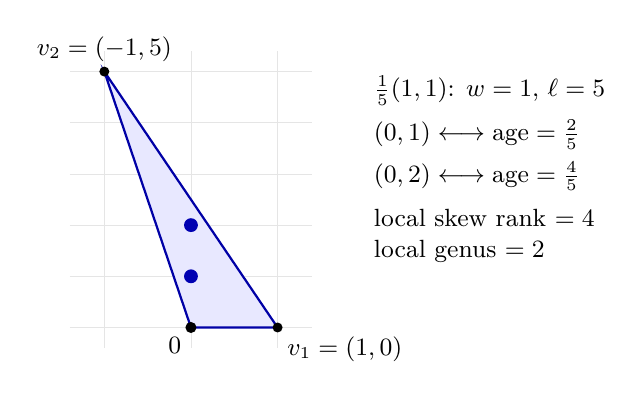
\begin{tikzpicture}[x=1.1cm,y=0.65cm,font=\small]
  \draw[step=1,gray!20,very thin] (-1.4,-0.4) grid (1.4,5.4);
  \filldraw[fill=blue!9,draw=blue!65!black,thick] (0,0)--(1,0)--(-1,5)--cycle;
  \fill (0,0) circle (2pt) node[below left] {$0$};
  \fill (1,0) circle (1.8pt) node[below right] {$v_1=(1,0)$};
  \fill (-1,5) circle (1.8pt) node[above] {$v_2=(-1,5)$};
  \fill[blue!70!black] (0,1) circle (2.5pt);
  \fill[blue!70!black] (0,2) circle (2.5pt);
  \node[anchor=west,align=left] at (2,3.1)
    {$\frac15(1,1)$: $w=1$, $\ell=5$\\[5pt]
     $(0,1)\longleftrightarrow\operatorname{age}=\frac25$\\[4pt]
     $(0,2)\longleftrightarrow\operatorname{age}=\frac45$\\[5pt]
     local skew rank $=4$\\
     local genus $=2$};
\end{tikzpicture}
\caption{The cone triangle for $\frac15(1,1)$ in the lattice $N=\Z^2$.  Its two interior points correspond to the two age-$<1$ sectors.  Each count equals the local genus contribution, not the total categorical genus.}
\label{fig:local-triangle}
\end{figure}

The lattice description is the usual age-simplex construction in the McKay correspondence.

\begin{definition}[Junior elements]
In the terminology of Ito--Reid, a stabilizer element is junior if its age is exactly one \cite[Section 1.2]{ItoReid}.
\end{definition}

We therefore say \emph{age less than one}, rather than \emph{junior}.  The vector space $H^{\operatorname{age}<1}_{\cX}$ has a basis indexed by the nontrivial sectors of age strictly less than one.

\begin{theorem}[Age interpretation]\label{thm:age-interpretation}
Let $X$ be a log del Pezzo surface with cyclic quotient singularities, and let $\cX$ be its canonical stack.  Its categorical genus satisfies
\begin{equation}\label{eq:age-genus}
\boxed{
g_{\mathrm{cat}}(\cX)=1+\dim H^{\operatorname{age}<1}_{\cX}.}
\end{equation}
\end{theorem}

\begin{proof}
For singularities $\frac1{n_j}(1,q_j)$, Lemma~\ref{lem:age-count} gives
\[
\dim H^{\operatorname{age}<1}_{\cX}
=\frac12\sum_j\bigl(n_j-\gcd(n_j,q_j+1)\bigr).
\]
Theorem~\ref{thm:cyclic-rank} identifies this sum with $g_{\mathrm{cat}}(\cX)-1$.
\end{proof}


\section{Residual singularities and mirror genus}\label{sec:mirror}

Lemma~\ref{lem:age-count} has identified half the local skew-rank contribution with both an age-$<1$ count and the interior lattice points of a cone triangle.  We now apply that identity to the residual cones of a toric degeneration, beginning with the relevant definitions.

\begin{definition}[Fano polygons]
A Fano polygon is a lattice polygon with primitive vertices and the origin strictly inside it.  The toric surface $X_P$ associated with a Fano polygon $P$ is defined by the fan over its edges, not by its normal fan.
\end{definition}

\begin{definition}[Maximally mutable Laurent polynomials]
A maximally mutable Laurent polynomial admits the prescribed algebraic mutations along polygon mutations: birational torus substitutions required to remain Laurent.  We use normalized vertex coefficients and zero constant term, with the mutability conventions of \cite[Section 3]{CKPT}.
\end{definition}

\begin{definition}[$\Q$-Gorenstein deformations]
A $\Q$-Gorenstein deformation is a deformation that locally comes from an equivariant deformation of the index-one cover, the cyclic cover on which the canonical class becomes Cartier.  This formulation includes the required base-change compatibility for reflexive powers of the relative canonical sheaf \cite[Basic Concepts]{ACC+}.
\end{definition}

\begin{definition}[Toric degenerations and local rigidity]
A toric $\Q$-Gorenstein degeneration of a del Pezzo surface is a $\Q$-Gorenstein degeneration with reduced fibers to a normal toric del Pezzo surface \cite[Definition 1]{ACC+}.  A surface is locally $\Q$-Gorenstein rigid if its singularities admit no nontrivial local $\Q$-Gorenstein deformations.
\end{definition}

\begin{definition}[Width and local Gorenstein index]
Consider a cyclic quotient $\frac1n(1,q)$.  Its cone has lattice width $w$ and lattice height $\ell$, equal to the local Gorenstein index (the height denoted $r$ in \cite[Basic Concepts]{ACC+}), determined by
\[
w=\gcd(n,q+1),\qquad n=w\ell.
\]
\end{definition}
Putting $a=(q+1)/w$ gives the useful normal form
\begin{equation}\label{eq:cyclic-normal-form}
\frac1{w\ell}(1,wa-1),\qquad \gcd(a,\ell)=1.
\end{equation}
The index-one cover is the hypersurface $xy=z^w$, with a residual $\mu_\ell$-action.  Its equivariant deformations describe the local $\Q$-Gorenstein deformations \cite[Basic Concepts]{ACC+}.

\begin{definition}[Smoothable and residual cyclic quotient singularities]
The decomposition into smoothable and residual parts is described by Euclidean division:
\[
w=m\ell+w_0,
\qquad 0\le w_0<\ell.
\]
The case $w_0=0$ gives a $T$-singularity, which is $\Q$-Gorenstein smoothable.  The case $m=0$, equivalently $0<w<\ell$, gives a residual singularity, which is $\Q$-Gorenstein rigid.  In general the residue keeps the same $a$ in \eqref{eq:cyclic-normal-form} and replaces $w$ by $w_0$:
\[
\frac1{w_0\ell}(1,w_0a-1)\quad(w_0>0);
\qquad\text{no residual point if }w_0=0.
\]
\end{definition}
Thus $m$ counts the primitive smoothable $T$-cones and $m\ell$ is the width occupied by the $T$-part.  A general local $\Q$-Gorenstein deformation removes this part \cite[Basic Concepts]{ACC+}.  A surface is locally $\Q$-Gorenstein rigid precisely when all its singularities are residual.  For example, $\frac13(1,1)$ and $\frac16(1,1)$ are residual, with $(w,\ell)=(1,3)$ and $(2,3)$, whereas $\frac14(1,1)$ is a $T$-singularity with $(w,\ell)=(2,2)$.

\begin{definition}[Singularity content]
The \emph{singularity content} of a Fano polygon is $(\sum m,\mathcal B)$, where the sum counts primitive $T$-cones and $\mathcal B$ is the multiset of its residual singularities.
\end{definition}

These conventions will also be used in Section~\ref{sec:qg-generic}, without redefining the local data.

The existence of a toric $\Q$-Gorenstein degeneration and local $\Q$-Gorenstein rigidity are independent conditions.  The surface $\Pj(1,1,4)$ is toric and hence admits such a degeneration, but is not locally $\Q$-Gorenstein rigid.  Conversely, the complete intersection $X_{6,6}\subset\Pj(2,2,3,3,3)$ has four residual $\frac13(1,1)$ points and degree $1/3$; it is the family $X_{4,1/3}$ in \cite[Section 7.6, entry 25]{OP}.  It is one of the three families without a toric $\Q$-Gorenstein degeneration: its anticanonical system is empty, whereas a toric surface has an effective anticanonical boundary, and $h^0(-K)$ is invariant in $\Q$-Gorenstein families \cite[Section 7]{CH}.

To apply Tveiten's genus formula, we express the residual singularities of a Fano polygon in terms of lattice points.

Figure~\ref{fig:mixed-cone-schematic} illustrates the separation of smoothable and residual contributions.

\begin{figure}[htbp]
\centering
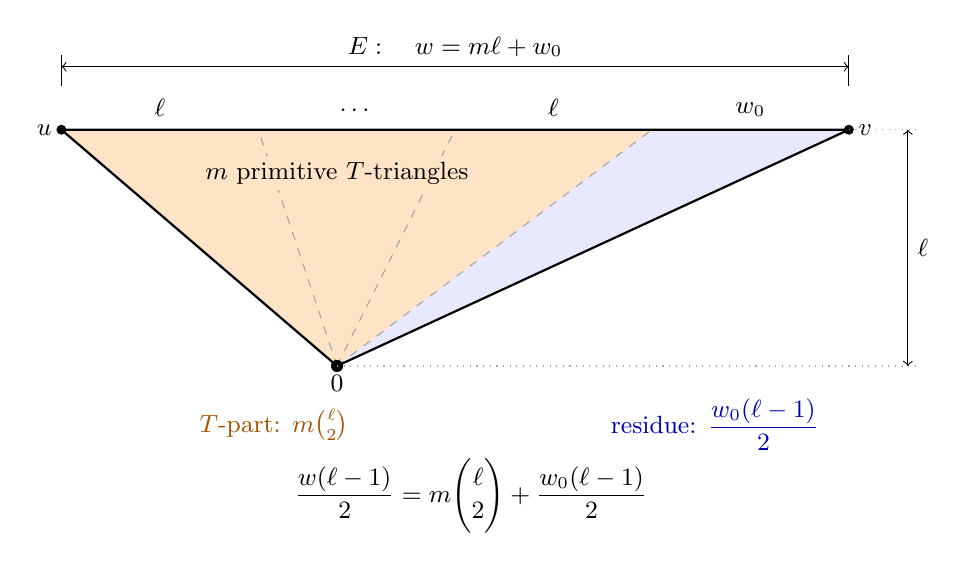
\begin{tikzpicture}[x=1cm,y=1cm,font=\small]
  \fill[orange!22] (3.5,0)--(0,3)--(7.5,3)--cycle;
  \fill[blue!9] (3.5,0)--(7.5,3)--(10,3)--cycle;
  \foreach \position in {2.5,5,7.5}
    \draw[gray!70,dashed] (3.5,0)--(\position,3);
  \draw[thick] (3.5,0)--(0,3)--(10,3)--cycle;
  \fill (3.5,0) circle (2.2pt) node[below] {$0$};
  \fill (0,3) circle (1.8pt) node[left] {$u$};
  \fill (10,3) circle (1.8pt) node[right] {$v$};
  \foreach \position/\width in {1.25/\ell,3.75/\cdots,6.25/\ell,8.75/w_0}
    \node[above] at (\position,3.05) {$\width$};
  \draw[thin] (0,3.55)--(0,3.95);
  \draw[thin] (10,3.55)--(10,3.95);
  \draw[<->] (0,3.8)--(10,3.8) node[midway,above] {$E:\quad w=m\ell+w_0$};
  \node[fill=orange!22,inner sep=2pt] at (3.5,2.45) {$m$ primitive $T$-triangles};
  \draw[gray!70,dotted] (3.5,0)--(10.9,0);
  \draw[gray!70,dotted] (10,3)--(10.9,3);
  \draw[<->] (10.75,0)--(10.75,3) node[midway,right] {$\ell$};
  \node[text=orange!65!black] at (2.7,-0.75) {$T$-part: $m\binom{\ell}{2}$};
  \node[text=blue!70!black] at (8.3,-0.75) {residue: $\dfrac{w_0(\ell-1)}2$};
  \node at (5.2,-1.65)
    {$\displaystyle\frac{w(\ell-1)}2=m\binom{\ell}{2}+\frac{w_0(\ell-1)}2$};
\end{tikzpicture}
\caption{Schematic decomposition of a mixed cone of width $w=m\ell+w_0$ and height $\ell$.  The orange part consists of $m$ primitive $T$-cones and contributes $m\binom{\ell}{2}$ to the categorical genus of the toric stack; the blue residual cone contributes $w_0(\ell-1)/2$ and survives a general $\Q$-Gorenstein deformation.  The repeated pieces are schematic, not a prescribed number of lattice triangles.}
\label{fig:mixed-cone-schematic}
\end{figure}

\begin{definition}[Residual lattice points]\label{def:residual-lattice-points}
Choose a crepant subdivision of the spanning fan of $P$ into primitive $T$-cones and residual cones $C_\alpha$: the inserted primitive ray generators lie on the original outer edge, so the canonical support function is unchanged and the induced toric morphism is crepant.  If $u_\alpha,v_\alpha$ are the primitive generators of $C_\alpha$, set
\[
R_{C_\alpha}
=\bigl(\operatorname{conv}\{0,u_\alpha,v_\alpha\}\cap N\bigr)
\setminus\{0,u_\alpha,v_\alpha\},
\qquad R=\bigcup_\alpha R_{C_\alpha}.
\]
\end{definition}
This is the residual set of \cite[Definitions 3.5--3.6]{CKPT}.  Here $R$ is a set of lattice points.  A mixed cone is subdivided first; only its residual subcone contributes to $R$.  The set $R$ itself may contain points of $\partial P$, but only $R\cap P^\circ$ enters the genus formula.  Primitive radial edges have no interior lattice points, so this intersection consists precisely of the interiors of the residual triangles.  Its cardinality is subdivision-independent: each residual triangle has width $w_0$ and height $\ell$ and contributes $w_0(\ell-1)/2$ by Lemma~\ref{lem:age-count}, regardless of where the $T$-part was cut.  Example~\ref{ex:mixed-cone-delta} exhibits two different residual sets with the same interior cardinality.  We use Tveiten's theorem \cite[Theorem 3.13]{Tveiten} in the following formulation \cite[Theorem 3.13]{CKPT}.

\begin{citedtheorem}[Tveiten's maximally mutable Laurent polynomial genus formula]
Let $f$ be a maximally mutable Laurent polynomial in two variables with Newton polygon $P$, and let $R$ be a choice of residual points as above.  Resolve the toric surface defined by the normal fan of $P$ and the basepoints of the pencil defined by $1$ and $f$.  The smooth projective model of a general member has genus
\[
g\bigl(\widetilde{\{f=\eta\}}\bigr)=1+\#(R\cap P^\circ).
\]
\end{citedtheorem}

The cited theorem does not require rigidity of the maximally mutable Laurent polynomial; ``general'' refers to the member of its pencil.  We use it for general polynomials in the relevant maximally mutable Laurent polynomial families, with the specified Newton polygon.

The polygon can be chosen without assuming a classification conjecture.  By hypothesis, choose a $\Q$-Gorenstein degeneration of $X$ to a toric surface $X_{P_0}$ and take its fan polygon $P_0$.  One may also replace $P_0$ by a mutation-equivalent polygon: mutation preserves the residual basket \cite[Theorem 3 and its proof]{ACC+}.  We do not require the conjectural injectivity of the assignment from mutation classes to $\Q$-Gorenstein deformation classes.

The basket equality is a local deformation statement.  In the normal form \eqref{eq:cyclic-normal-form}, the index-one cover deforms as $xy=z^{w_0}F(z^\ell)$, with $F$ a monic polynomial of degree $m$.  A root at zero of multiplicity $b$ retains a point of width $w_0+b\ell$ with the same residue; multiple nonzero roots produce only smoothable Du Val points.  Thus a nongeneral fiber can still have mixed singularities, not merely a disjoint union of residual and $T$-singularities.  On a locally $\Q$-Gorenstein rigid fiber, however, all remaining smoothable parts must vanish.  Its basket is therefore exactly the residual basket of $P_0$, and hence of $P$ \cite[Basic Concepts; Lemma 6 and proof of Theorem 3]{ACC+}.

\begin{theorem}[The locally rigid mirror-genus comparison]\label{cor:genus-match}

Let $X$ be a locally $\Q$-Gorenstein rigid log del Pezzo surface with cyclic quotient singularities admitting a toric $\Q$-Gorenstein degeneration, let $\cX$ be its canonical stack, and choose a $\Q$-Gorenstein degeneration to $X_{P_0}$.  Let $P$ be $P_0$ or a mutation-equivalent Fano polygon.  For a general maximally mutable Laurent polynomial $f$ with Newton polygon $P$ and a general value $\eta$, the smooth projective model of the fiber satisfies
\[
\boxed{
g_{\mathrm{cat}}(\cX)
=g\bigl(\widetilde{\{f=\eta\}}\bigr).}
\]
\end{theorem}

\begin{proof}
By the preceding local argument, the singularities of $X$ are the residues of the cones of $P$.  Lemma~\ref{lem:age-count} identifies the contribution of each residual triangle with its age-$<1$ count and local categorical genus correction.  Summing gives
\[
\#(R\cap P^\circ)=\dim H^{\operatorname{age}<1}_{\cX}.
\]
The maximally mutable Laurent polynomial genus formula \cite[Theorem 3.13]{CKPT} and Theorem~\ref{thm:age-interpretation} now yield
\[
g\bigl(\widetilde{\{f=\eta\}}\bigr)
=1+\#(R\cap P^\circ)
=g_{\mathrm{cat}}(\cX).
\]
\end{proof}

\begin{remark}\label{rem:local-rigidity-needed}
For $\Pj(1,1,4)$, Proposition~\ref{prop:weighted-rank} gives $g_{\mathrm{cat}}=2$, but its $\frac14(1,1)$ point is $\Q$-Gorenstein smoothable and contributes no residual point, so a general maximally mutable Laurent polynomial fiber has genus one.  Thus local $\Q$-Gorenstein rigidity cannot simply be dropped from the comparison with the given stack.  The categorical and age formulas remain valid; Section~\ref{sec:qg-generic} instead compares maximally mutable Laurent polynomial genus with the generic $\Q$-Gorenstein deformation.
\end{remark}

For the Corti--Heuberger families discussed in the introduction, Theorem~\ref{cor:genus-match} identifies the categorical value $k+1$ with mirror genus whenever the family admits a toric $\Q$-Gorenstein degeneration.  Remark~\ref{rem:smooth-blowup} also shows that this value is constant along smooth-locus blow-ups in their cascades.

\begin{example}[The $X_{10}$ mirror polygon]\label{ex:x10-mirror-polygon}
For $X_{10}$, the case $r=1$ gives $g_{\mathrm{cat}}(\cX_{10})=2$.  Its mirror mutation class contains
\[
P=\operatorname{conv}\{(-3,-5),(-3,5),(7,5)\},
\]
with singularity content $(10,\{\frac13(1,1)\})$ \cite[Table 4 and Theorem 9]{KNP}.  Here $10$ counts primitive $T$-cones and the residual basket consists of one $\frac13(1,1)$ point.  The general maximally mutable Laurent polynomial fiber has genus two, matching $g_{\mathrm{cat}}(\cX_{10})=2$.  Proposition~\ref{prop:x10-explicit-model} derives the explicit hyperelliptic model from the Laurent polynomial in \cite[Section 7.3, entry 11]{OP}.
\end{example}

Figure~\ref{fig:x10-subdivision} separates the residual point from the smoothable content; Example~\ref{ex:x10-toric-drop} computes the resulting drop of $34$.
\begin{figure}[htbp]
\centering
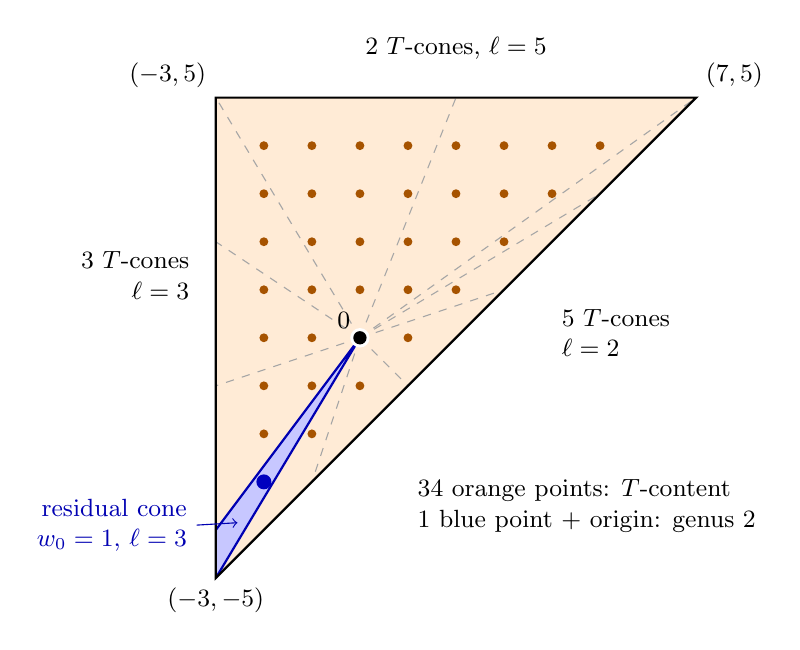
\begin{tikzpicture}[x=0.61cm,y=0.61cm,font=\small]
  \fill[orange!16] (-3,-5)--(7,5)--(-3,5)--cycle;
  \fill[blue!22] (0,0)--(-3,-4)--(-3,-5)--cycle;
  \foreach \horizontal/\vertical in {-3/-5,-1/-3,1/-1,3/1,5/3,7/5,2/5,-3/5,-3/2,-3/-1,-3/-4}
    \draw[gray!70,dashed,thin] (0,0)--(\horizontal,\vertical);
  \draw[blue!70!black,thick] (-3,-4)--(0,0)--(-3,-5);
  \draw[thick] (-3,-5)--(7,5)--(-3,5)--cycle;
  \foreach \horizontal/\lowest in {-2/-3,-1/-2,0/-1,1/0,2/1,3/2,4/3,5/4}
    \foreach \vertical in {\lowest,...,4}
      \fill[orange!65!black] (\horizontal,\vertical) circle (1.6pt);
  \fill[blue!75!black] (-2,-3) circle (2.7pt);
  \fill[white] (0,0) circle (3.5pt);
  \fill (0,0) circle (2.4pt) node[above left] {$0$};
  \node[above left] at (-3,5) {$(-3,5)$};
  \node[above right] at (7,5) {$(7,5)$};
  \node[below] at (-3,-5) {$(-3,-5)$};
  \node[above,align=center] at (2,5.6) {$2$ $T$-cones, $\ell=5$};
  \node[anchor=east,align=right] at (-3.35,1.3) {$3$ $T$-cones\\$\ell=3$};
  \node[anchor=west,align=left] at (4,0.1) {$5$ $T$-cones\\$\ell=2$};
  \node[anchor=east,align=right,text=blue!70!black] at (-3.4,-3.9) {residual cone\\$w_0=1$, $\ell=3$};
  \draw[blue!70!black,->] (-3.4,-3.9)--(-2.55,-3.85);
  \node[anchor=west,align=left] at (1,-3.5)
    {$34$ orange points: $T$-content\\
     $1$ blue point $+$ origin: genus $2$};
\end{tikzpicture}
\caption{A crepant subdivision of the $X_{10}$ mirror polygon into ten primitive $T$-cones (orange) and one residual cone (blue).  The $36$ interior points comprise $34$ points in the $T$-triangles, one residual point, and the origin.  Thus the toric canonical stack has categorical genus $36$, while the residual and maximally mutable Laurent polynomial genera are $2$.}
\label{fig:x10-subdivision}
\end{figure}

The polygon has substantial smoothable $T$-content.  What happens to categorical genus when that content is removed?  The next section answers this question under general $\Q$-Gorenstein deformation and identifies the surviving value with mirror genus.

\section{\texorpdfstring{$\Q$-Gorenstein}{Q-Gorenstein} deformation and the mirror-side genus drop}\label{sec:qg-generic}

Section~\ref{sec:mirror} distinguishes the categorical genus of the given canonical stack, which retains both residual and smoothable local contributions, from the maximally mutable Laurent polynomial genus, which retains only the residual part.  The categorical object to compare with the mirror is therefore the canonical stack of a sufficiently general $\Q$-Gorenstein deformation.  What survives this deformation, and where does the discarded genus appear on the compactified mirror curve?  We answer the first question by the residual formula and the exact $T$-content drop, neither of which requires a toric degeneration.  With a toric degeneration, the surviving value is mirror genus; under the boundary hypotheses below, the discarded part is the total boundary $\delta$-invariant.

\begin{lemma}[The generic residual basket]\label{lem:generic-residual-basket}
Let $X$ be a log del Pezzo surface with cyclic quotient singularities.  A sufficiently small miniversal $\Q$-Gorenstein deformation $\mathfrak X\to(B,0)$, with $X_0=X$, has a smooth irreducible base germ and a nonempty open locus $B^\circ$ on which the fibers $X_t$ have exactly the residual basket of $X$.  After shrinking $B$, these fibers remain log del Pezzo.
\end{lemma}

\begin{proof}
By \cite[Lemma 6]{ACC+}, $\Q$-Gorenstein deformations of $X$ are unobstructed and restriction to the product of the local deformation functors is formally smooth.  On miniversal base germs this gives a smooth, hence dominant, map to the product of the smooth local bases.  The local normal form in \eqref{eq:cyclic-normal-form} has a dense open deformation locus removing all $T$-content and keeping exactly its residue.  The inverse image of the product of these loci is nonempty and open in the irreducible global base.  Openness of ampleness keeps the fibers log del Pezzo after shrinking, and smoothness away from neighborhoods of the original singularities prevents additional singular points.  This gives the required locus $B^\circ$.
\end{proof}

\begin{definition}[Categorical genus under general $\Q$-Gorenstein deformation]\label{def:qg-generic-genus}
Choose a miniversal family $\mathfrak X\to(B,0)$ as in Lemma~\ref{lem:generic-residual-basket}.  For $t\in B^\circ$, let $\mathcal X_t$ denote the canonical stack of the fiber $X_t$.  Define
\[
g_{\mathrm{cat}}^{\mathrm{qG}}(X)
=g_{\mathrm{cat}}^{\mathrm{res}}(X)
:=g_{\mathrm{cat}}(\mathcal X_t).
\]
The superscripts $\mathrm{res}$ and $\mathrm{qG}$ indicate, respectively, the residual basket and the $\Q$-Gorenstein deformation used to compute the invariant.
\end{definition}

A sufficiently general deformation removes all $T$-content and retains exactly the residual basket, by Lemma~\ref{lem:generic-residual-basket}.  Theorem~\ref{thm:cyclic-rank} therefore makes the value independent of the general member and the miniversal realization, with no choice of a local deformation component.  This concerns the miniversal germ at $X$, not components of a global moduli space.  The numerical consequence is the following residual formula.

\begin{proposition}[Residual formula]\label{prop:qg-residual-genus}
Let $X$ be a cyclic quotient log del Pezzo surface, and use the local data $(w_j,\ell_j,m_j,w_{0,j})$ of Section~\ref{sec:mirror} at its singular points.  The categorical genus under general $\Q$-Gorenstein deformation is
\begin{equation}\label{eq:qg-generic-genus}
\boxed{g_{\mathrm{cat}}^{\mathrm{qG}}(X)
=1+\frac12\sum_j w_{0,j}(\ell_j-1).}
\end{equation}
\end{proposition}

\begin{proof}
Use the normal form \eqref{eq:cyclic-normal-form}, with $a=(q+1)/w$ and $\gcd(a,\ell)=1$.  Lemma~\ref{lem:generic-residual-basket} removes the $m\ell$-part of the width, leaving the residue with the same $a$:
\[
\frac1{w_0\ell}(1,w_0a-1)
\quad\text{if }w_0>0,
\]
and there is no residual point if $w_0=0$.  This is a reduced cyclic quotient: since $w_0a-1\equiv wa-1=q\pmod\ell$, it is coprime to $\ell$, and $w_0a-1\equiv-1\pmod{w_0}$ shows that it is also coprime to $w_0$.  The greatest common divisor determining its width is
\[
\gcd(w_0\ell,w_0a)=w_0.
\]
Theorem~\ref{thm:cyclic-rank} therefore gives local genus contribution
$(w_0\ell-w_0)/2=w_0(\ell-1)/2$.  Summing over the generic residual basket proves \eqref{eq:qg-generic-genus}.
\end{proof}

Thus $g_{\mathrm{cat}}^{\mathrm{qG}}$ is obtained from the cyclic basket formula simply by replacing each width $w_j$ by its residual width $w_{0,j}$.  The remaining contribution measures precisely the categorical genus lost when the smoothable $T$-content is removed.

\begin{corollary}[The $T$-content drop]\label{cor:t-content-drop}
For a cyclic quotient log del Pezzo surface $X$, with the notation of Proposition~\ref{prop:qg-residual-genus}, one has
\begin{equation}\label{eq:t-content-drop}
\boxed{g_{\mathrm{cat}}(\cX)-g_{\mathrm{cat}}^{\mathrm{qG}}(X)
=\sum_j m_j\binom{\ell_j}{2}.}
\end{equation}
Equivalently, for $t\in B^\circ$ in Lemma~\ref{lem:generic-residual-basket}, the ranks of the skew Euler forms of $\cX$ and the canonical stack $\mathcal X_t$ of $X_t$ satisfy
\[
\boxed{\rk_{\Q}\chi^-_{\cX}-\rk_{\Q}\chi^-_{\mathcal X_t}
=\sum_j m_j\ell_j(\ell_j-1).}
\]
\end{corollary}

\begin{proof}
Theorem~\ref{thm:cyclic-rank} gives local genus correction
$(n_j-w_j)/2=w_j(\ell_j-1)/2$ on $\cX$, whereas Proposition~\ref{prop:qg-residual-genus} gives $w_{0,j}(\ell_j-1)/2$ on the generic stack.  Their difference is
\[
\frac{w_j(\ell_j-1)}2-\frac{w_{0,j}(\ell_j-1)}2
=\frac{m_j\ell_j(\ell_j-1)}2
=m_j\binom{\ell_j}{2}.
\]
Summing proves \eqref{eq:t-content-drop}; doubling gives the skew-rank formula.
\end{proof}

The corollary separates the categorical genus into its surviving residual term and the exact contribution of the smoothable $T$-content:
\[
\boxed{g_{\mathrm{cat}}(\cX)
=g_{\mathrm{cat}}^{\mathrm{qG}}(X)+\sum_jm_j\binom{\ell_j}{2}.}
\]
The categorical side is now completely separated into a deformation-invariant residual contribution and a smoothable contribution.  Residual points have $m_j=0$ and leave the genus unchanged; at a pure $T$-singularity, $w_{0,j}=0$, so the entire local contribution disappears.  In particular, a $\frac14(1,1)$ point has $(m,\ell)=(1,2)$ and contributes a drop of $1$.  This gives $g_{\mathrm{cat}}^{\mathrm{qG}}(\Pj(1,1,4))=1$ and explains the drop of $2$ in Petracci's example.

The preceding formulas are intrinsic to $X$.  When $X$ is toric, both pieces acquire a lattice interpretation.  We first count all interior lattice points of the full polygon, before removing any $T$-content.

\begin{proposition}[Toric categorical genus]\label{prop:toric-categorical-genus}
Let $P\subset N_{\mathbb R}$ be a Fano polygon in a rank-two lattice $N$, and let $X_P$ be the toric del Pezzo surface whose fan consists of the cones over the faces of $P$.  Its canonical stack satisfies
\begin{equation}\label{eq:toric-categorical-genus}
\boxed{g_{\mathrm{cat}}(\mathcal X_P)=\#(P^\circ\cap N).}
\end{equation}
\end{proposition}

\begin{proof}
Order the primitive vertices $v_1,\dots,v_r$ counterclockwise, with $v_{r+1}=v_1$, and put $\Delta_i=\operatorname{conv}\{0,v_i,v_{i+1}\}$.  The cone over the $i$th edge has determinant $n_i>0$, edge width $w_i$, and local Gorenstein index $\ell_i$, with $n_i=w_i\ell_i$.  For a singular cone of type $\frac1{n_i}(1,q_i)$, its width is $w_i=\gcd(n_i,q_i+1)$.  For a smooth cone we take $n_i=w_i=\ell_i=1$, so its local correction is zero.

Lemma~\ref{lem:age-count} gives $\#(\Delta_i^\circ\cap N)=(n_i-w_i)/2$, the local genus correction in Theorem~\ref{thm:cyclic-rank}; for a smooth cone both numbers are zero.  The triangles cover $P$ and meet along radial segments.  Such a segment contains no lattice points other than $0$ and its primitive endpoint, which lies on $\partial P$.  Thus every nonzero lattice point in $P^\circ$ belongs to exactly one triangle interior.  The origin is itself an interior lattice point of the Fano polygon and contributes the initial $1$.  Consequently
\[
\#(P^\circ\cap N)
=1+\sum_i\frac{n_i-w_i}{2}
=g_{\mathrm{cat}}(\mathcal X_P).
\]
\end{proof}

\begin{remark}[A toric numerical consistency check]\label{rem:toric-numerical-check}
In the setting of Proposition~\ref{prop:toric-categorical-genus}, let $r$ be the number of rays and $n_i$ the cone determinants, including $n_i=1$ for smooth cones.  The toric divisor sequence gives $\rho(X_P)=r-2$ \cite[Theorem 4.1.3 and Proposition 4.2.7]{CLS}.  Proposition~\ref{prop:numerical-inertia} and the untwisted decomposition in Lemma~\ref{lem:untwisted-rank} therefore give
\[
\dim_{\Q}K_0^{\mathrm{num}}(\mathcal X_P)_{\Q}
=2+(r-2)+\sum_{i=1}^r(n_i-1)
=\sum_{i=1}^r n_i=2\operatorname{Area}_N(P),
\]
where a fundamental parallelogram of $N$ has area one.  This uses the canonical stack, with no generic or divisorial stabilizers.  Writing $I=\#(P^\circ\cap N)$ and $B=\#(\partial P\cap N)$, Proposition~\ref{prop:toric-categorical-genus} and Pick's theorem yield
\[
\rk_{\Q}\chi^-_{\mathcal X_P}=2I,
\qquad
2\operatorname{Area}_N(P)=2I+B-2.
\]
By Lemma~\ref{lem:skew-serre}, the kernel on numerical $K$-theory consequently satisfies
\[
\dim_{\Q}\ker(1-S_{\mathcal X_P})=B-2.
\]
Together with the general Laurent-polynomial genus in Corollary~\ref{cor:toric-laurent-genus}, these identities provide a numerical consistency check for the comparison between the Euler and Seifert pairings \cite[Sections 4.2 and 5]{HarderThompson}.
\end{remark}

The same full interior-lattice-point count gives the genus of a general Laurent-polynomial fiber, providing the first bridge from categorical genus to curve geometry.

\begin{corollary}[General Laurent-polynomial fibers]\label{cor:toric-laurent-genus}
With $P$ as in Proposition~\ref{prop:toric-categorical-genus}, let $h\in\C[N]$ be a general Laurent polynomial with Newton polygon $P$.  For general $\eta$, the smooth projective model of its fiber satisfies
\[
\boxed{g_{\mathrm{cat}}(\mathcal X_P)
=g\bigl(\widetilde{\{h=\eta\}}\bigr).}
\]
\end{corollary}

\begin{proof}
For general coefficients and $\eta$, the polynomial $h-\eta$ is nondegenerate with respect to $P$: for each face, including $P$ itself, its face polynomial and logarithmic partial derivatives have no common zero in the torus.  A general member is irreducible by Bertini for the toric linear system of the two-dimensional polygon $P$.  For its smooth projective model $C$, Khovanskii's formula \cite[Section 1, Theorem 1]{KhovanskiiGenus} gives $\chi(\mathcal O_C)=1-\#(P^\circ\cap N)$, hence
$g(C)=\#(P^\circ\cap N)$.  Proposition~\ref{prop:toric-categorical-genus} identifies this with categorical genus.
\end{proof}

Here the curve is compactified using the normal fan of its Newton polygon, distinct from the fan over the faces of $P$ defining $X_P$.  Maximal mutability changes the genus count: a general Laurent polynomial records all interior lattice points, whereas a general maximally mutable Laurent polynomial records only the residual interior points together with the origin.  It is therefore the residual categorical genus that enters the mirror comparison.

\begin{corollary}[$\Q$-Gorenstein generic mirror genus]\label{cor:qg-generic-mirror-genus}
Let $X$ be a cyclic quotient log del Pezzo surface admitting a toric $\Q$-Gorenstein degeneration, and choose $X_t$ as in Lemma~\ref{lem:generic-residual-basket}.  Let $P$ be a Fano polygon whose residual basket agrees with that of $X_t$; in particular one may use a polygon of a chosen toric $\Q$-Gorenstein degeneration of $X$, or a mutation-equivalent polygon.  For a general maximally mutable Laurent polynomial $f$ with Newton polygon $P$ and general $\eta$, one has
\begin{equation}\label{eq:qg-generic-mirror-genus}
\boxed{g_{\mathrm{cat}}^{\mathrm{qG}}(X)
=1+\#(R\cap P^\circ)
=g\bigl(\widetilde{\{f=\eta\}}\bigr),}
\end{equation}
where $R$ is the residual set of $P$.
\end{corollary}

\begin{proof}
By Proposition~\ref{prop:qg-residual-genus}, the left-hand side is $1+\frac12\sum_jw_{0,j}(\ell_j-1)$.  By Lemma~\ref{lem:age-count}, each nonempty residue contributes exactly $w_{0,j}(\ell_j-1)/2$ interior residual points.  The basket hypothesis identifies their sum with $\#(R\cap P^\circ)$, and the maximally mutable Laurent polynomial genus formula \cite[Theorem 3.13]{CKPT} proves the remaining equality.
\end{proof}

This completes the mirror comparison in Theorem~\ref{thm:intro-mirror}.  Equation~\eqref{eq:qg-generic-mirror-genus} identifies the categorical residual basket, the residual lattice-point count, and the genus of a general maximally mutable Laurent-polynomial fiber as three descriptions of the same quantity.

\begin{remark}[Choice of toric degeneration]\label{rem:choice-of-toric-degeneration}
Theorem~3 of \cite{ACC+} gives a surjection from polygon mutation classes to $\Q$-Gorenstein deformation classes of locally $\Q$-Gorenstein rigid surfaces admitting toric $\Q$-Gorenstein degenerations.  The deformation input is Lemma~6 of \cite{ACC+}: unobstructedness and formal smoothness of the global-to-local deformation map, together with the local residual smoothing, give the generic residual basket, as in Lemma~\ref{lem:generic-residual-basket}.  This is the mechanism used in the proof of \cite[Theorem 3]{ACC+} to pass to locally rigid members.  Consequently, the sufficiently general deformations associated with any two toric degenerations of $X$ have the residual basket of a sufficiently general deformation of $X$, and Corollary~\ref{cor:qg-generic-mirror-genus} gives the same mirror genus for both.  No mutation equivalence of the two polygons is required: injectivity of the surjection is the separate assertion of Conjecture~A in \cite{ACC+} and is not used here.
\end{remark}

The numerical loss in Corollary~\ref{cor:t-content-drop} raises a geometric question: where does the genus disappear on the mirror curve?  The categorical calculation measures how much is lost, and Corollary~\ref{cor:qg-generic-mirror-genus} identifies what survives with mirror genus.  The mirror-side defect itself is already present in Tveiten's local discussion.

Tveiten observes that when $m$ mutation factors on an edge of height $\ell$ coincide, the resulting point is not an ordinary $m\ell$-fold point: it is an $\ell$-fold point whose branches have order-$m$ tangency, with total genus defect $m\binom{\ell}{2}$ \cite[Remark 3.14, arXiv version 2]{Tveiten}.  The same remark notes that special fibers such as $f=0$ may have smaller genus when the constant coefficient vanishes.  Our comparison uses a general member $f=\eta$, for which the constant coefficient of $f-\eta$ is $-\eta$.

Lutz describes the corresponding boundary basepoints.  His mutable cycle records the points and multiplicities prescribed by mutation factors \cite[Definition 3.1]{Lutz}; Theorem~3.3 and Corollary~3.4 of \cite{Lutz} identify the associated sections after successive boundary blow-ups, subtracting the edge height $h_E=\ell_E$ from each exceptional class.  For the normalized $T$-part, the $m_E$ successive centers lie over $x=-1$; after the first blow-up they are infinitely near, at intersections of the strict boundary transform with the new exceptional divisor.  Lemma~3.2 of \cite{Lutz} gives the weighted local vanishing and multiplicity at least $\ell_E$ at each center.  Equality holds for general fibers under the hypotheses below.  We use this general construction, not the elliptic-fibration conclusion for $T$-polygons whose pencil is resolved in \cite[Lemma 3.6]{Lutz}.  Proposition~\ref{prop:boundary-delta} makes the geometry explicit in the normalized maximally mutable Laurent-polynomial coordinates used here and identifies its $\delta$-invariant with the independently computed categorical $\Q$-Gorenstein genus drop.

\begin{samepage}
For $m>0$ and $\ell>1$, the hypotheses of Proposition~\ref{prop:boundary-delta} give the chain
\[
\boxed{\begin{gathered}
\text{maximal mutability}\Longrightarrow\text{mutable boundary data}\\
\Longrightarrow\text{$m$ successive boundary centers of multiplicity $\ell$}\\
\Longrightarrow\text{boundary singularity}\Longrightarrow\delta=m\binom{\ell}{2}.
\end{gathered}}
\]
\end{samepage}
For $\ell=1$, the point is smooth and contributes zero.  Figure~\ref{fig:boundary-delta} illustrates the geometry under the proposition's hypotheses.  The proof below derives the local invariant from slice divisibility and identifies it with the categorical contribution computed in Corollary~\ref{cor:t-content-drop}.

\begin{figure}[!htbp]
\centering
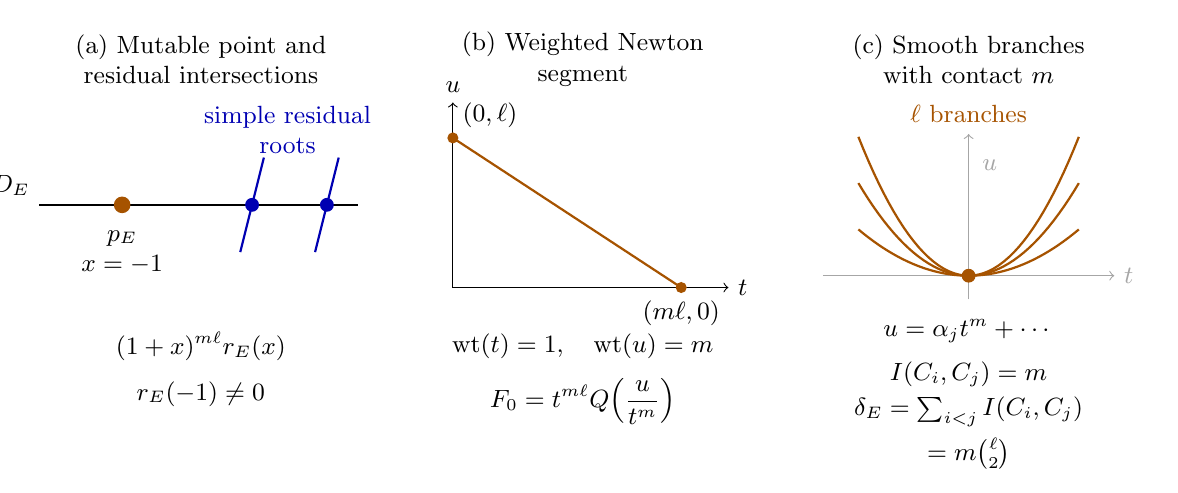
\begin{tikzpicture}[x=1cm,y=1cm,font=\small]
  \useasboundingbox (-0.15,-2.05) rectangle (14.1,3.5);
  \begin{scope}
    \node[align=center] at (2.05,3.1) {(a) Mutable point and\\residual intersections};
    \draw[thick] (0,1.25)--(4.05,1.25);
    \node[above left] at (0,1.25) {$D_E$};
    \foreach \position in {2.7,3.65} {
      \draw[blue!70!black,thick] (\position-0.15,0.65)--(\position+0.15,1.85);
      \fill[blue!70!black] (\position,1.25) circle (2.5pt);
    }
    \fill[orange!65!black] (1.05,1.25) circle (3pt);
    \node[below,align=center] at (1.05,1.05) {$p_E$\\$x=-1$};
    \node[text=blue!70!black,align=center] at (3.15,2.2) {simple residual\\roots};
    \node at (2.05,-0.55) {$(1+x)^{m\ell}r_E(x)$};
    \node at (2.05,-1.15) {$r_E(-1)\ne0$};
  \end{scope}
  \begin{scope}[xshift=4.9cm]
    \node[align=center] at (2,3.1) {(b) Weighted Newton\\segment};
    \draw[->] (0.35,0.2)--(3.85,0.2) node[right] {$t$};
    \draw[->] (0.35,0.2)--(0.35,2.55) node[above] {$u$};
    \draw[orange!65!black,thick] (0.35,2.1)--(3.25,0.2);
    \fill[orange!65!black] (0.35,2.1) circle (2pt);
    \fill[orange!65!black] (3.25,0.2) circle (2pt);
    \node[above right] at (0.35,2.1) {$(0,\ell)$};
    \node[below] at (3.25,0.15) {$(m\ell,0)$};
    \node at (2,-0.55) {$\operatorname{wt}(t)=1,\quad\operatorname{wt}(u)=m$};
    \node at (2,-1.25) {$F_0=t^{m\ell}Q\!\left(\dfrac{u}{t^m}\right)$};
  \end{scope}
  \begin{scope}[xshift=9.8cm]
    \node[align=center] at (2,3.1) {(c) Smooth branches\\with contact $m$};
    \draw[gray!70,->] (0.15,0.35)--(3.85,0.35) node[right] {$t$};
    \draw[gray!70,->] (2,0.05)--(2,2.15);
    \node[gray!70,anchor=west] at (2.05,1.75) {$u$};
    \foreach \coefficient in {0.3,0.6,0.9}
      \draw[orange!65!black,thick,domain=-1.4:1.4,samples=45]
        plot ({2+\x},{0.35+\coefficient*\x*\x});
    \fill[orange!65!black] (2,0.35) circle (2.5pt);
    \node[text=orange!65!black] at (2,2.4) {$\ell$ branches};
    \node at (2,-0.35) {$u=\alpha_jt^m+\cdots$};
    \node at (2,-0.9) {$I(C_i,C_j)=m$};
    \node[align=center] at (2,-1.65)
      {$\delta_E=\sum_{i<j}I(C_i,C_j)$\\[3pt]$=m\binom{\ell}{2}$};
  \end{scope}
\end{tikzpicture}
\caption{Boundary geometry of the $T$-content, schematically and under the hypotheses of Proposition~\ref{prop:boundary-delta}.  The smoothable edge factor is concentrated at the orange point $x=-1$.  The weighted Newton segment produces $\ell$ smooth branches with pairwise intersection multiplicity $m$, hence $\delta_E=m\binom{\ell}{2}$.  The blue residual roots meet the boundary transversely.  Panel (c) uses three representative tangent branches to illustrate $m>1$, not a fixed value of $\ell$.}
\label{fig:boundary-delta}
\end{figure}

\begin{samepage}
\begin{proposition}[$T$-content as a boundary $\delta$-invariant]\label{prop:boundary-delta}
Let $P$ be a Fano polygon and let $f$ belong to the normalized maximally mutable family of \cite[Propositions 3.7 and 3.9]{CKPT}.  For each edge $E$, write $w_E=m_E\ell_E+w_{0,E}$, with $0\le w_{0,E}<\ell_E$.  Up to a monomial, write its edge polynomial as $(1+x)^{m_E\ell_E}r_E(x)$ in a primitive edge coordinate.  Assume that every residual factor $r_E$ has simple roots, that $r_E(-1)\ne0$ whenever $m_E>0$, and that the general fiber is irreducible.

Let $\overline C_\eta$ be the closure of $f=\eta$ on the toric surface defined by the normal fan of $P$.  For general $\eta$ and each edge with $m_E>0$, the point $x=-1$ on its boundary divisor has $\ell_E$ smooth branches with pairwise intersection multiplicity $m_E$.  Its local invariant, with $\delta_E=0$ for $m_E=0$, is
\[
\boxed{\delta_E=m_E\binom{\ell_E}{2}.}
\]
These are the only possible singularities of $\overline C_\eta$, and
\[
\boxed{
g_{\mathrm{cat}}(\mathcal X_P)-g\bigl(\widetilde{\overline C_\eta}\bigr)
=\sum_E\delta_E=\sum_E m_E\binom{\ell_E}{2}.}
\]
\end{proposition}
\end{samepage}



\begin{proof}
Fix an edge with $m=m_E>0$ and $\ell=\ell_E$.  Choose torus coordinates in which this edge lies at height $\ell$, and write $f=\sum_h f_h(x)y^h$.  Proposition~3.7 of \cite{CKPT} prescribes mutability with factor $(1+x)^m$, and Proposition~3.9 identifies this family with the maximally mutable family.  The substitution $y\mapsto y/(1+x)^m$ is Laurent precisely when $(1+x)^{mh}$ divides $f_h(x)$ for every $h>0$.  This is the slice condition we use, not an assertion that coincident mutable points are ordinary multiple points.

At the boundary point, $t=x+1$ and $u=y^{-1}$ are smooth local coordinates.  Multiplying $f-\eta$ by $u^\ell$ and a monomial unit gives an equation $F(t,u)=0$.  The slice condition and $r_E(-1)\ne0$ imply that its lowest part for weights $\operatorname{wt}(t)=1$, $\operatorname{wt}(u)=m$ is
\[
F_0(t,u)=\sum_{i=0}^{\ell}c_i t^{m(\ell-i)}u^i
=t^{m\ell}Q(u/t^m),\qquad c_0\ne0.
\]
The coefficient $c_\ell$ varies affinely and nontrivially with $\eta$; the other $c_i$ are fixed.  Thus $Q$ has degree $\ell$ and distinct nonzero roots for general $\eta$: a repeated root would give a critical value of the nonconstant rational function $\bigl(\sum_{i<\ell}c_i z^i\bigr)/z^\ell$, of which there are only finitely many.  In particular the Newton segment joins $(m\ell,0)$ to $(0,\ell)$.

Substituting $u=t^mz$ and dividing by $t^{m\ell}$ gives $Q(z)+tH(t,z)=0$ with $H$ analytic.  The implicit function theorem at each root $\alpha_j$ gives a branch
\[
u=\alpha_jt^m+O(t^{m+1}),\qquad j=1,\ldots,\ell.
\]
All branches are smooth, and distinct leading coefficients give intersection multiplicity $m$ for every pair.  Additivity of $\delta$ over the branches therefore yields $\delta_E=m\binom\ell2$.

The torus part is smooth outside the finitely many critical values of $f$.  Simple residual roots give transverse boundary intersections, and nonzero vertex coefficients keep the curve away from toric fixed points.  Hence there are no other singularities.  The toric arithmetic-genus formula gives $p_a(\overline C_\eta)=\#(P^\circ\cap N)=g_{\mathrm{cat}}(\mathcal X_P)$ by Proposition~\ref{prop:toric-categorical-genus}.  The normalization formula $p_a-g=\sum\delta$ proves the stated identity and identifies it with the drop in Corollary~\ref{cor:t-content-drop}.
\end{proof}

\begin{samepage}
For the toric surface $X_P$, take $f$ satisfying Proposition~\ref{prop:boundary-delta} and a general value $\eta$, and retain its notation $\overline C_\eta$ for the compactified fiber.  Proposition~\ref{prop:toric-categorical-genus}, Corollary~\ref{cor:qg-generic-mirror-genus}, and the boundary calculation identify
\[
\begin{aligned}
g_{\mathrm{cat}}(\mathcal X_P)&=p_a(\overline C_\eta),\\
g_{\mathrm{cat}}^{\mathrm{qG}}(X_P)&=g\bigl(\widetilde{\overline C_\eta}\bigr)=g_{\mathrm{MMLP}}.
\end{aligned}
\]
The exact deformation drop is therefore the arithmetic genus lost on normalization:
\[
\boxed{\begin{aligned}
g_{\mathrm{cat}}(\mathcal X_P)-g_{\mathrm{cat}}^{\mathrm{qG}}(X_P)
&=p_a(\overline C_\eta)-g\bigl(\widetilde{\overline C_\eta}\bigr)\\
&=\sum_E\delta_E=\sum_E m_E\binom{\ell_E}{2}.
\end{aligned}}
\]
Thus the same quantity is measured in three ways: as $g_{\mathrm{cat}}(\mathcal X_P)-g_{\mathrm{cat}}^{\mathrm{qG}}(X_P)$, as the $T$-content discarded in passing from all interior lattice points to the mutable genus $1+\#(R\cap P^\circ)$, and as the total boundary $\delta$-invariant $\sum_E\delta_E$.  Under the stated hypotheses, the categorical genus lost under $\Q$-Gorenstein deformation equals the mirror genus defect described by Tveiten and realized through Lutz's successive boundary blow-ups.
\end{samepage}

\section{Examples and explicit mirror checks}\label{sec:explicit-mirrors}

The general comparison is now established.  We begin the explicit checks with the motivating $X_{10}$ mirror and then consider the other Oneto--Petracci families.

We write $X_{k,d}$ for a surface with $k$ points of type $\frac13(1,1)$ and anticanonical degree $d=K_X^2$, following \cite[Section 7]{OP}.  For such a surface, Proposition~\ref{prop:third-rank} gives $\rk\chi^-=2k+2$ and $g_{\mathrm{cat}}=k+1$.  For the families admitting toric $\Q$-Gorenstein degenerations, the mirror polygon has $k$ residual cones of this type, so Theorem~\ref{cor:genus-match} already predicts genus $k+1$.  The purpose here is different: we exhibit that genus directly in representative Laurent-polynomial mirrors from Oneto--Petracci \cite[Section 7]{OP}.  These computations are not inputs to the categorical theorem.  They test its terminology on models constructed independently through period calculations.

We use one representative for each value $k=1,2,3,4,6$ occurring in their explicit period computations.  The value $k=5$ is absent because the quantum period of $X_{5,5/3}$ is not computed there: a suitable toric complete-intersection or quotient model was unavailable \cite[Introduction and Theorem 2.2]{OP}.  This is only a gap in the Oneto--Petracci period calculations, not in the toric degeneration or maximally mutable Laurent polynomial description; Example~\ref{ex:five-point-toric} supplies the genus-$6$ comparison without quantum periods.  All section numbers, numbered entries, and polygon drawings cited here follow the publisher version of Oneto--Petracci \cite[Section 7]{OP}, not the first arXiv version.  In particular, the six-point surface $X_{6,2}$ is entry~26 in Section~7.7.  Some entries specify only a subfamily of the maximally mutable Laurent polynomial parameter space; we distinguish these from a general maximally mutable Laurent polynomial with the full polygon.  In each calculation, genus means the genus of the smooth projective model.  To exclude additional singularities in the torus, we use the following generic-smoothness observation: a nonconstant Laurent polynomial over $\C$ has only finitely many critical values, since it is constant on each irreducible component of its critical locus.  Thus its general fiber is smooth in $(\C^*)^2$, and it remains to check the boundary of the compactification.

For $k=1$, the representative $X_{10}=X_{1,1/3}$ is entry~11 of \cite[Section 7.3, polygon 1]{OP}.  Their notation $a_{[p,q]}$ means the coefficient of the monomial $x^py^q$.  The displayed mirror specialization is
\[
f_{360}(x,y)=x^{-3}y^5(1+x+y^{-1})^{10}-2520,
\qquad a_{[4,3]}=360.
\]
The following proposition proves the genus directly, including a one-parameter Laurent-polynomial extension of this specialization.  We do not claim that the extension exhausts the normalized maximally mutable Laurent polynomial parameter space.

\begin{proposition}[The explicit $X_{10}$ genus-two model]\label{prop:x10-explicit-model}
Put $H=1+x+y^{-1}$ and define
\begin{equation}\label{eq:x10-factorized-family}
f_a=x^{-3}y^5H^{10}-2520+(a-360)(x^{-2}y^3H^6-60).
\end{equation}
Its Newton polygon is the triangle $P$ of Example~\ref{ex:x10-mirror-polygon}, its constant term is zero, and $[x^4y^3]f_a=a$.  Set $s=a-360$ and let $\lambda=\eta+2520+60s$ be the shifted fiber value.  For general $(s,\lambda)$, the fiber $f_a=\eta$ is birational to
\begin{equation}\label{eq:x10-hyperelliptic}
v^2=-\lambda(u+s)\left(4u^3(u+s)^2-\lambda u^2(u+s)+4\lambda^2\right).
\end{equation}
Its smooth projective model has genus two.  The same conclusion holds for $a=360$ and general $\eta$.
\end{proposition}

\begin{proof}
The constant terms of $x^{-3}y^5H^{10}$ and $x^{-2}y^3H^6$ are, respectively,
\[
\frac{10!}{3!5!2!}=2520,\qquad \frac{6!}{2!3!1!}=60.
\]
Their coefficients of $x^4y^3$ are $10!/(7!2!1!)=360$ and $1$.  This proves the normalization.  The first summand has the three vertices of $P$ with coefficients one, and the support of the second lies strictly inside $P$, so the Newton polygon is unchanged.

On the fiber introduce
\[
u=x^{-1}y^2H^4,\qquad A=x^{-2}y^3H^6.
\]
Then $x^{-3}y^5H^{10}=Au$ and
\[
A(u+s)=\lambda,\qquad x=\frac{u^3}{A^2},\qquad yH^2=\frac{u^2}{A}.
\]
Thus $A=\lambda/(u+s)$ and $x=u^3(u+s)^2/\lambda^2$.  Set $B=1+x$; the identity $H=B+y^{-1}$ gives
\[
B^2y^2+\left(2B-\frac{u^2}{A}\right)y+1=0.
\]
Its discriminant $\Delta=u^4/A^2-4Bu^2/A$ satisfies
\[
\frac{\lambda^4}{u^2}\Delta
=-\lambda(u+s)\left(4u^3(u+s)^2-\lambda u^2(u+s)+4\lambda^2\right).
\]
Taking $v=(\lambda^2/u)(2B^2y+2B-u^2/A)$ yields \eqref{eq:x10-hyperelliptic}.  Conversely,
\[
y=\frac{uv/\lambda^2-2B+u^2/A}{2B^2}
\]
recovers $y$ rationally, and the preceding identities recover $x,u,A$ on dense open sets.  This proves birationality.  The minus sign is the one obtained from the discriminant; replacing $v$ by $iv$ over $\C$ gives the opposite-sign quadratic twist.

For $\lambda\ne0$ the right-hand side has degree six.  At $(s,\lambda)=(0,1)$ it equals $-uQ(u)$, where $Q(u)=4u^5-u^3+4$.  Since $Q(0)=4$ and $Q'(u)=u^2(20u^2-3)$, a common root $\alpha$ of $Q$ and $Q'$ would satisfy $\alpha^2=3/20$.  Substituting this into $Q(\alpha)=0$ gives $4-3\alpha/50=0$, hence $\alpha=200/3$, a contradiction.  Thus $Q$ is squarefree and coprime to $u$, so the sextic is squarefree.  Squarefreeness is open, so it holds for general $(s,\lambda)$ and also for general $\lambda$ on $s=0$.  The resulting double cover of $\Pj^1$ has six branch points; Riemann--Hurwitz gives genus two.
\end{proof}

For $k=2$, use the one-parameter mirror of $X_{2,8/3}$ in \cite[Section 5.3; Section 7.4, entry 15, polygon 13]{OP}:
\[
f_a(x,y)=\frac{(1+x+y)^3}{xy}+xy+a(x+y)-6.
\]
Writing $c=\eta+6$, clearing denominators gives $(1+x+y)^3+x^2y^2+a xy(x+y)-cxy=0$.  Its closure in $\Pj^2$ is the quartic
\begin{equation}\label{eq:op-quartic}
F_{a,c}=z(z+x+y)^3+x^2y^2+a xyz(x+y)-c xyz^2=0.
\end{equation}
To verify smoothness, take $a=0$, $c=1$.  On $z=0$ the curve meets only $[1:0:0]$ and $[0:1:0]$, and $F_z$ is nonzero at both.  On $z=1$, put $G=(1+x+y)^3+x^2y^2-xy$.  At a singular point,
\[
G_x-G_y=(y-x)(2xy-1)=0.
\]
If $2xy=1$, the equations $G_x=G_y=0$ force $1+x+y=0$, but then $G=-1/4$.  Otherwise $x=y=t$, and $G=G_x=0$ would give a common root of
\[
p(t)=t^4+8t^3+11t^2+6t+1,
\qquad q(t)=2t^3+12t^2+11t+3.
\]
Here $q=p'/2$, so $\operatorname{Res}_t(p,q)=\operatorname{disc}(p)/16=-89\ne0$.  This checks all projective Jacobian equations.  Smoothness is open in the projective family \eqref{eq:op-quartic}, so its general member is a smooth, necessarily irreducible plane quartic.  It follows that
\[
g=\frac{(4-1)(4-2)}2=3=g_{\mathrm{cat}}.
\]

For $k=3$, \cite[Section 7.5, entry 20, polygon 14]{OP} gives the following specialization for $X_{3,3}$, with $a_{[0,1]}=a_{[-1,0]}=0$ and $a_{[-1,1]}=1$:
\[
f(x,y)=\frac{x}{y}\left(1+\frac1x+y\right)^2
+\frac yx\left(1+\frac1x+y\right)-2.
\]
Set $L=x+1+xy$ and $c=\eta+2$.  Clearing denominators gives $xL^2+y^2L-cx^2y=0$, whose quintic homogenization is
\[
H=x(xz+z^2+xy)^2+zy^2(xz+z^2+xy)-cx^2yz^2=0.
\]
The affine boundary points are $(0,0)$ and $(-1,0)$; their respective nonzero derivatives are $H_x=1$ and $H_y=-c$ in the chart $z=1$.  At infinity the only points are $A=[0:1:0]$ and $B=[1:0:0]$.  In the chart $y=1$ at $A$, the quadratic part is $xz$, so $A$ is an ordinary node.  In the chart $x=1$ at $B$, the quadratic part is $(y+z)^2$, and restriction to its double tangent gives
\[
H(1,-z,z)=cz^3+z^4+z^5.
\]
For $c\ne0$ this is an $A_2$ cusp: after completing the square in the transverse coordinate $y+z$, the first nonzero term along the tangent has degree three.  Both singularities have $\delta=1$.  The generic-smoothness observation excludes further singularities for general $c$.  No coordinate line is a component, since
\[
H|_{z=0}=x^3y^2,\qquad H|_{x=0}=y^2z^3,\qquad
H|_{y=0}=xz^2(x+z)^2
\]
are all nonzero polynomials.  The quintic is also irreducible: a reduced reducible quintic without a boundary component would have, by B\'ezout, intersection multiplicity at least $1\cdot4=4$ between its components, exceeding the total $\delta$-invariant two.  Therefore
\[
g=\frac{(5-1)(5-2)}2-1-1=4=g_{\mathrm{cat}}.
\]
This specialization retains the full polygon~14.  Thus, unlike the six-point expression discussed below, it already realizes the genus predicted for the general maximally mutable Laurent polynomial.

For $k=4$, choose $X_{4,4/3}$, entry~24 of \cite[Section 7.6]{OP}.  Its polygon~5 is the octagon with vertices $(\pm2,\pm1)$ and $(\pm1,\pm2)$, with all sign choices.  The four horizontal and vertical edges have binomial coefficients $1,2,1$.  Together with the interior coefficients specified in that entry, they give
\begin{equation}\label{eq:op-four-polynomial}
\begin{aligned}
f_a(x,y)={}&(x^2+x^{-2})(y+2+y^{-1})
+(y^2+y^{-2})(x+2+x^{-1})\\
&+(a+8)(x+x^{-1})(y+y^{-1})
+(2a+14)(x+x^{-1}+y+y^{-1}).
\end{aligned}
\end{equation}
Multiplying $f_a-\eta$ by $x^2y^2$ and bihomogenizing gives a curve $C$ of bidegree $(4,4)$ in $\Pj^1\times\Pj^1$.  Since $K_{\Pj^1\times\Pj^1}=\mathcal O(-2,-2)$ and $(a,b)\cdot(c,d)=ad+bc$, adjunction gives
\[
2p_a(C)-2=(4,4)\cdot(2,2)=16,
\qquad p_a(C)=9.
\]
On $x=0$ its equation restricts to $y(y+1)^2$; inversion of either coordinate and interchange of $x,y$ give the other boundary charts.  The four corners are smooth, with local linear part $x+y$ at $(0,0)$.  The only remaining boundary points are
\[
(0,-1),\quad(\infty,-1),\quad(-1,0),\quad(-1,\infty).
\]
At the first, in coordinates $u=x$, $v=y+1$, the quadratic part is
\[
-v^2-(\eta+4a+24)u^2.
\]
It has distinct tangent lines when $\eta+4a+24\ne0$; the symmetries give the same conclusion at all four points.  They are therefore ordinary nodes, and a general fiber has no additional singularities in the torus.

To prove irreducibility, we use the following change of variables.  Put $U=x+x^{-1}+2$, $V=y+y^{-1}+2$ and $b=\eta+4a+24$.  The fiber equation becomes
\[
UV(U+V+a)=b.
\]
Its plane cubic closure is smooth for general $(a,b)$.  The two quadratic equations recovering $x$ and $y$ have discriminants $U(U-4)$ and $V(V-4)$.  On the cubic, the first has simple zeros at the two affine points with $U=4$; the third intersection of the projective line $U=4$ with the cubic is the point at infinity $[0:1:0]$.  At each of these two affine points the second discriminant is a unit for general parameters, and the analogous statement holds with $U,V$ interchanged.  A square in a function field has even valuation at every point.  These simple zeros show that neither discriminant, nor their product, is a square, so their square classes are independent.  Adjoining both square roots gives a degree-four field extension, proving irreducibility of the $(4,4)$ curve.  Consequently its normalization has
\[
g=9-4=5=g_{\mathrm{cat}}.
\]

For $k=6$, use the family with the specified Newton polygon for $X_{6,2}$ associated with polygon~9 in \cite[Section 7.7, entry 26]{OP}:
\begin{equation}\label{eq:op-six-polygon}
P_6=\operatorname{conv}\{(1,-2),(2,-1),(1,1),(-1,2),(-2,1),(-1,-1)\}.
\end{equation}

\begin{remark}[The printed polynomial]\label{rem:printed-polynomial}
The expression printed in this entry omits $xy$, although $(1,1)$ is a vertex of the specified Newton polygon.  The opposite vertex monomial $x^{-1}y^{-1}$ is present with coefficient one.  Restoring $xy$ with coefficient one therefore adds $2$ to the contribution of the antipodal vertex pairs to the constant term of $f^2$, changing that vertex contribution from $4$ to $6$.  This is consistent with the printed coefficient of $t^2$ in the period and supports a typographical omission; by itself it does not verify the full period.  We use the family with the specified Newton polygon below.
\end{remark}

\begin{definition}[Nondegenerate Laurent equations]
A Laurent equation is \emph{nondegenerate with respect to its polygon} if every face polynomial, including the whole polynomial, has no common torus zero with its logarithmic partial derivatives.
\end{definition}

For a nondegenerate curve, the adjunction formula $p_a(C)=1+(C^2+C\cdot K)/2$ on a smooth toric compactification gives the number of interior Newton lattice points \cite[Section 1, Theorem 1]{KhovanskiiGenus}.

With vertex coefficients normalized to one, write the family as
\[
f_{\boldsymbol a}=\frac{x}{y^2}+\frac{x^2}{y}+xy+\frac{y^2}{x}
+\frac y{x^2}+\frac1{xy}
+a_1x+a_2y+a_3\frac yx+a_4\frac1x+a_5\frac1y+a_6\frac xy.
\]
Every edge of $P_6$ has width one and height three; hence all six cones are residual $\frac13(1,1)$ cones, and there are no $T$-mutability constraints.  The six edge determinants are all three, giving area nine, while all six edges are primitive, so the total lattice boundary length, equivalently the boundary lattice-point count, is six.  Pick's theorem yields
\[
\#(P_6^\circ\cap\Z^2)=9-\frac62+1=7.
\]
Each edge polynomial is a primitive binomial with a simple root.  The closure on the toric surface of the normal fan therefore meets the boundary transversely and avoids its fixed points; for general parameters and fiber value it is also smooth in the torus.  Toric adjunction gives arithmetic genus $1+(18-6)/2=7$.  This smooth ample curve is connected, hence irreducible, so its geometric genus is seven.

\begin{proposition}[Explicit mirror check]\label{prop:explicit-mirror-check}
For the representative Oneto--Petracci subfamilies computed above for $X_{1,1/3}$, $X_{2,8/3}$, $X_{3,3}$, $X_{4,4/3}$, and the restored family with the specified Newton polygon for $X_{6,2}$, the genus of a general fiber agrees with categorical genus as follows:
\[
\begin{array}{c|c|c}
k&g_{\mathrm{cat}}&g(\text{general fiber in the subfamily})\\\hline
1&2&2\\2&3&3\\3&4&4\\4&5&5\\6&7&7
\end{array}
\]
\end{proposition}

\begin{proof}
The preceding compactifications give the displayed genera directly on the indicated representatives.  Theorem~\ref{cor:genus-match} gives the same genera for general maximally mutable Laurent polynomials in their mutation classes, while Proposition~\ref{prop:third-rank} gives the categorical values.
\end{proof}

These checks are independent confirmations on mirror models constructed by period calculations rather than from the Euler pairing.  They realize half the ranks of the skew Euler pairings, namely $2,3,4,5,7$, as ordinary geometric genera and make the numerical comparison concrete.

\begin{example}[Cavey--Prince polygons]\label{ex:cavey-prince}
To test other residual singularities, consider the polygons
\[
P=\operatorname{conv}\{(0,1),(-k_1,-1),(k_2,-1)\}
\]
of Cavey--Prince \cite[Proposition 7.1 and Remark 7.2]{CP}, with $(k_1,k_2)=(3,6)$ or $(5,5)$.  Their toric surfaces admit $\Q$-Gorenstein deformations to $X_{k_1+k_2}\subset\Pj(1,1,k_1,k_2)$, with residual basket $\frac1{k_1}(1,1),\frac1{k_2}(1,1)$.  For explicit curve checks we use the binomial specialization
\[
f_{k_1,k_2}(x,y)=y+\frac{(1+x)^{k_1+k_2}}{x^{k_1}y}.
\]
This polynomial has Newton polygon $P$; we obtain it by choosing the binomial coefficients along the horizontal edge in the polygon construction of \cite{CP}.

For $X_9\subset\Pj(1,1,3,6)$, the $\frac13(1,1)$ point contributes $1$, while the $\frac16(1,1)$ point has $w=2$, $\ell=3$, and contributes $2$.  Hence $g_{\mathrm{cat}}=1+1+2=4$.  On $f_{3,6}=\eta$, set $v=x^2(2y-\eta)$.  Clearing denominators gives
\[
v^2=P_{10}(x):=\eta^2x^4-4x(1+x)^9.
\]
For $X_{10}\subset\Pj(1,1,5,5)$, each of the two $\frac15(1,1)$ points contributes $2$, so $g_{\mathrm{cat}}=1+2+2=5$.  On $f_{5,5}=\eta$, the substitution $v=x^3(2y-\eta)$ gives
\[
v^2=P_{11}(x):=\eta^2x^6-4x(1+x)^{10}.
\]
At $\eta=1$, direct polynomial division gives $\gcd(P_{10},P_{10}')=\gcd(P_{11},P_{11}')=1$; squarefreeness therefore holds for general $\eta$.  The smooth projective models have genera $4$ and $5$, respectively.  The genus-$4$ curve provides an explicit mirror-curve check with residual width $w_0=2$, testing Lemma~\ref{lem:age-count} beyond width $1$; the second independently checks the $\frac15(1,1)$ contribution.  Cavey--Prince's cascade polygons and Laurent polynomials provide analogous examples with a single singular point for arbitrary $k$ \cite[Table 8.1]{CP}.
\end{example}

\begin{example}[Separate residual and smoothable cones]\label{ex:petracci-drop}
Petracci's toric surface makes the distinction following Theorem~\ref{cor:genus-match} quantitative: rigid and smoothable contributions coexist, and the latter account exactly for the difference between the categorical genus of the given canonical stack and that of the canonical stack of a general $\Q$-Gorenstein deformation.

Let $X_P$ be the toric del Pezzo surface with polygon
\[
P=\operatorname{conv}\{(2,1),(1,2),(-1,2),(-2,-1),(-1,-2),(1,-2)\}.
\]
Petracci \cite[Proposition 2.1]{PetracciKmoduli} proves that it is K-polystable and has basket
\[
2\times\tfrac13(1,1),\qquad
2\times\tfrac14(1,1),\qquad
2\times\tfrac15(1,2).
\]
The first and third types are $\Q$-Gorenstein rigid.  The two $\frac14(1,1)$ points admit simultaneous global $\Q$-Gorenstein smoothings: the global $\Q$-Gorenstein deformation functor has hull $\C[\![t_1,t_2]\!]$, with independent smoothing parameters, and Petracci realizes it by an explicit family \cite[Section 2.2, equation (5), Proposition 2.3(B), and Section 2.5]{PetracciKmoduli}.  Write $X_t$ for a sufficiently general fiber of this family and $\mathcal X_t$ for its canonical stack.  Its basket is
\[
2\times\tfrac13(1,1)+2\times\tfrac15(1,2).
\]
Theorem~\ref{thm:cyclic-rank} assigns local genus corrections $1$, $1$, and $2$ to $\frac13(1,1)$, $\frac14(1,1)$, and $\frac15(1,2)$, respectively: the relevant gcds are $1$, $2$, and $1$.  Consequently
\[
g_{\mathrm{cat}}(\mathcal X_P)=1+2\cdot1+2\cdot1+2\cdot2=9,
\qquad
g_{\mathrm{cat}}(\mathcal X_t)=1+2\cdot1+2\cdot2=7.
\]
Figure~\ref{fig:petracci-hexagon} displays the two smoothable contributions and the six residual points.
\begin{figure}[htbp]
\centering
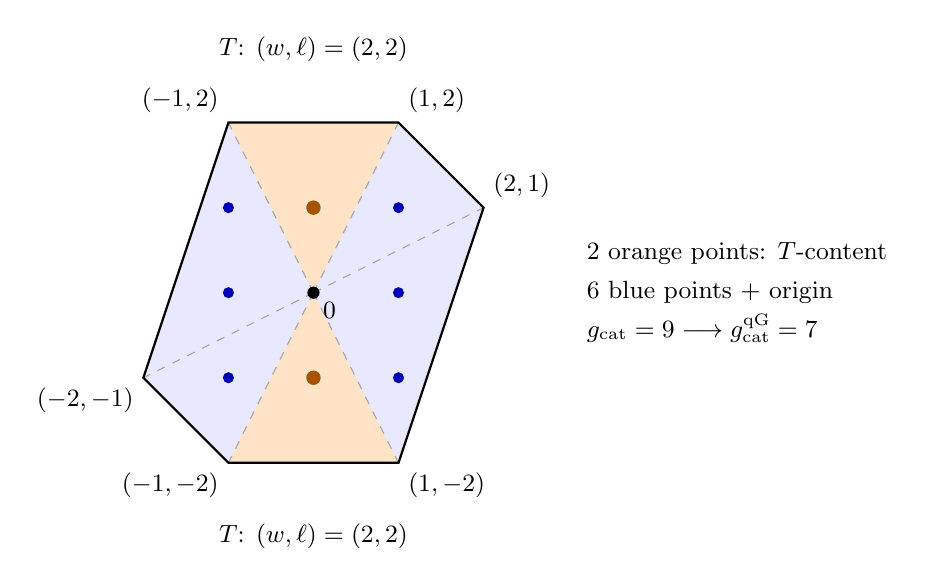
\begin{tikzpicture}[x=1.08cm,y=1.08cm,font=\small]
  \fill[blue!9] (2,1)--(1,2)--(-1,2)--(-2,-1)--(-1,-2)--(1,-2)--cycle;
  \fill[orange!22] (0,0)--(1,2)--(-1,2)--cycle;
  \fill[orange!22] (0,0)--(-1,-2)--(1,-2)--cycle;
  \foreach \horizontal/\vertical in {2/1,1/2,-1/2,-2/-1,-1/-2,1/-2}
    \draw[gray!70,dashed] (0,0)--(\horizontal,\vertical);
  \draw[thick] (2,1)--(1,2)--(-1,2)--(-2,-1)--(-1,-2)--(1,-2)--cycle;
  \foreach \horizontal in {-1,1}
    \foreach \vertical in {-1,0,1}
      \fill[blue!70!black] (\horizontal,\vertical) circle (2pt);
  \foreach \vertical in {-1,1}
    \fill[orange!65!black] (0,\vertical) circle (2.6pt);
  \fill (0,0) circle (2.2pt) node[below right] {$0$};
  \node[above] at (0,2.6) {$T$: $(w,\ell)=(2,2)$};
  \node[below] at (0,-2.6) {$T$: $(w,\ell)=(2,2)$};
  \node[above right] at (2,1) {$(2,1)$};
  \node[above right] at (1,2) {$(1,2)$};
  \node[above left] at (-1,2) {$(-1,2)$};
  \node[below left] at (-2,-1) {$(-2,-1)$};
  \node[below left] at (-1,-2) {$(-1,-2)$};
  \node[below right] at (1,-2) {$(1,-2)$};
  \node[anchor=west,align=left] at (3.1,0)
    {$2$ orange points: $T$-content\\[3pt]
     $6$ blue points $+$ origin\\[3pt]
     $g_{\mathrm{cat}}=9\longrightarrow g_{\mathrm{cat}}^{\mathrm{qG}}=7$};
\end{tikzpicture}
\caption{Petracci's hexagon, with its two $T$-cones shaded orange.  Each contains one interior lattice point; the four residual cones contain six points in total.  Keeping these six points and the origin gives the residual genus $7$, compared with the categorical genus of the original toric stack $9$.}
\label{fig:petracci-hexagon}
\end{figure}

Petracci \cite[Section 3.2]{PetracciKmoduli} gives the explicit maximally mutable Laurent polynomial family
\[
\begin{aligned}
f={}&x^2y+x^{-2}y^{-1}+(x+2+x^{-1})(y^2+y^{-2})\\
&+a_1xy+a_2x^{-1}y^{-1}+b_1x+b_2x^{-1}
+c_1xy^{-1}+c_2x^{-1}y.
\end{aligned}
\]
The two width-two, height-two cones are pure $T$-cones.  The remaining four residual cones contribute $1,1,2,2$ interior residual points.  Thus the maximally mutable Laurent polynomial genus formula \cite[Theorem 3.13]{CKPT} gives
\[
\boxed{g_{\mathrm{cat}}(\mathcal X_P)=9,\qquad
g_{\mathrm{cat}}(\mathcal X_t)=7,\qquad
g_{\mathrm{MMLP}}=7.}
\]
The drop $9-7=2$ is exactly the contribution of the two smoothed $\frac14(1,1)$ points.  This is the passage to the generic residual basket described in Lemma~\ref{lem:generic-residual-basket}.
\end{example}

\begin{example}[A mixed cone with residual width $2$]\label{ex:mixed-cone-delta}
Consider the polygon
\[
\boxed{P=\operatorname{conv}\{(-1,3),(4,3),(0,-1)\}.}
\]
Figure~\ref{fig:mixed-cone-example} shows the polygon, its two residual subdivisions, and the mutation described below.

\begin{figure}[tp]
\centering
\begin{minipage}[t]{0.49\textwidth}
\centering
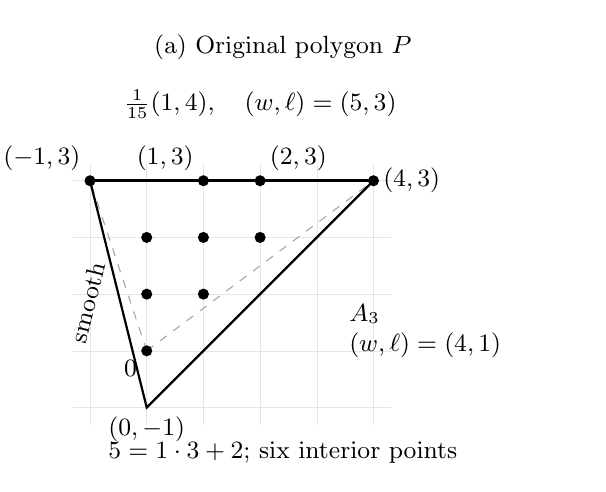
\begin{tikzpicture}[x=0.72cm,y=0.72cm,font=\small]
  \useasboundingbox (-2.1,-2) rectangle (7.6,5.7);
  \node at (2.4,5.35) {(a) Original polygon $P$};
  \draw[step=1,gray!20,very thin] (-1.3,-1.3) grid (4.3,3.3);
  \draw[gray!70,dashed] (0,0)--(-1,3) (0,0)--(4,3);
  \draw[thick] (-1,3)--(4,3)--(0,-1)--cycle;
  \draw[line width=1.1pt] (-1,3)--(4,3);
  \foreach \horizontal/\vertical in {0/0,0/1,0/2,1/1,1/2,2/2}
    \fill (\horizontal,\vertical) circle (2pt);
  \foreach \horizontal in {-1,1,2,4}
    \fill (\horizontal,3) circle (2pt);
  \node[above left] at (-1,3) {$(-1,3)$};
  \node[above left] at (1,3) {$(1,3)$};
  \node[above right] at (2,3) {$(2,3)$};
  \node[right] at (4,3) {$(4,3)$};
  \node[below] at (0,-1) {$(0,-1)$};
  \node[below left] at (0,0) {$0$};
  \node at (2,4.35) {$\frac1{15}(1,4),\quad(w,\ell)=(5,3)$};
  \node[align=left,anchor=west] at (3.4,0.35) {$A_3$\\$(w,\ell)=(4,1)$};
  \node[rotate=76] at (-1.05,0.85) {smooth};
  \node at (2.4,-1.8) {$5=1\cdot3+2$; six interior points};
\end{tikzpicture}
\end{minipage}\hfill
\begin{minipage}[t]{0.49\textwidth}
\centering
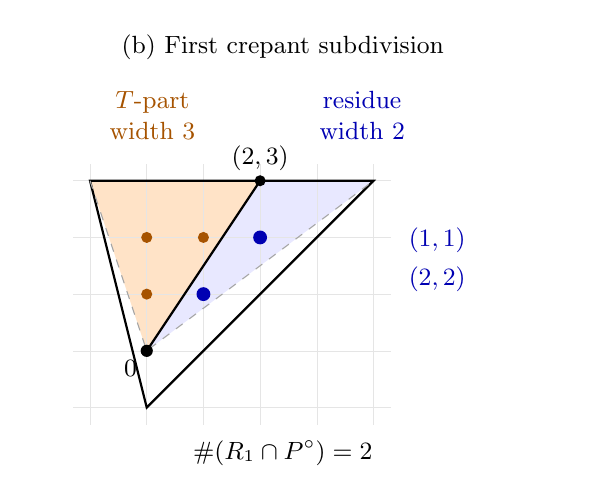
\begin{tikzpicture}[x=0.72cm,y=0.72cm,font=\small]
  \useasboundingbox (-2.1,-2) rectangle (7.6,5.7);
  \node at (2.4,5.35) {(b) First crepant subdivision};
  \fill[orange!22] (0,0)--(-1,3)--(2,3)--cycle;
  \fill[blue!9] (0,0)--(2,3)--(4,3)--cycle;
  \draw[step=1,gray!20,very thin] (-1.3,-1.3) grid (4.3,3.3);
  \draw[thick] (-1,3)--(4,3)--(0,-1)--cycle;
  \draw[gray!70,dashed] (-1,3)--(0,0)--(4,3);
  \draw[thick] (0,0)--(2,3);
  \foreach \horizontal/\vertical in {0/1,0/2,1/2}
    \fill[orange!65!black] (\horizontal,\vertical) circle (2pt);
  \foreach \horizontal/\vertical in {1/1,2/2}
    \fill[blue!70!black] (\horizontal,\vertical) circle (2.5pt);
  \fill (0,0) circle (2.2pt) node[below left] {$0$};
  \fill (2,3) circle (2pt) node[above] {$(2,3)$};
  \node[text=orange!65!black,align=center] at (0.1,4.15) {$T$-part\\width $3$};
  \node[text=blue!70!black,align=center] at (3.8,4.15) {residue\\width $2$};
  \node[text=blue!70!black,anchor=west,align=left] at (4.45,1.6) {$(1,1)$\\[3pt]$(2,2)$};
  \node at (2.4,-1.8) {$\#(R_1\cap P^\circ)=2$};
\end{tikzpicture}
\end{minipage}

\medskip
\begin{minipage}[t]{0.49\textwidth}
\centering
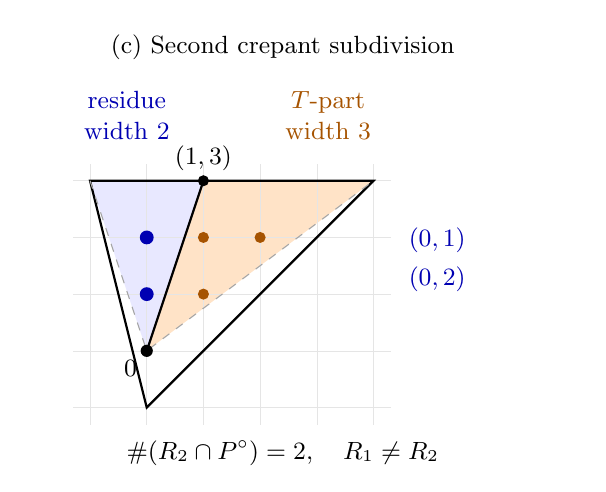
\begin{tikzpicture}[x=0.72cm,y=0.72cm,font=\small]
  \useasboundingbox (-2.1,-2) rectangle (7.6,5.7);
  \node at (2.4,5.35) {(c) Second crepant subdivision};
  \fill[blue!9] (0,0)--(-1,3)--(1,3)--cycle;
  \fill[orange!22] (0,0)--(1,3)--(4,3)--cycle;
  \draw[step=1,gray!20,very thin] (-1.3,-1.3) grid (4.3,3.3);
  \draw[thick] (-1,3)--(4,3)--(0,-1)--cycle;
  \draw[gray!70,dashed] (-1,3)--(0,0)--(4,3);
  \draw[thick] (0,0)--(1,3);
  \foreach \horizontal/\vertical in {1/1,1/2,2/2}
    \fill[orange!65!black] (\horizontal,\vertical) circle (2pt);
  \foreach \vertical in {1,2}
    \fill[blue!70!black] (0,\vertical) circle (2.5pt);
  \fill (0,0) circle (2.2pt) node[below left] {$0$};
  \fill (1,3) circle (2pt) node[above] {$(1,3)$};
  \node[text=blue!70!black,align=center] at (-0.35,4.15) {residue\\width $2$};
  \node[text=orange!65!black,align=center] at (3.2,4.15) {$T$-part\\width $3$};
  \node[text=blue!70!black,anchor=west,align=left] at (4.45,1.6) {$(0,1)$\\[3pt]$(0,2)$};
  \node at (2.4,-1.8) {$\#(R_2\cap P^\circ)=2,\quad R_1\ne R_2$};
\end{tikzpicture}
\end{minipage}\hfill
\begin{minipage}[t]{0.49\textwidth}
\centering
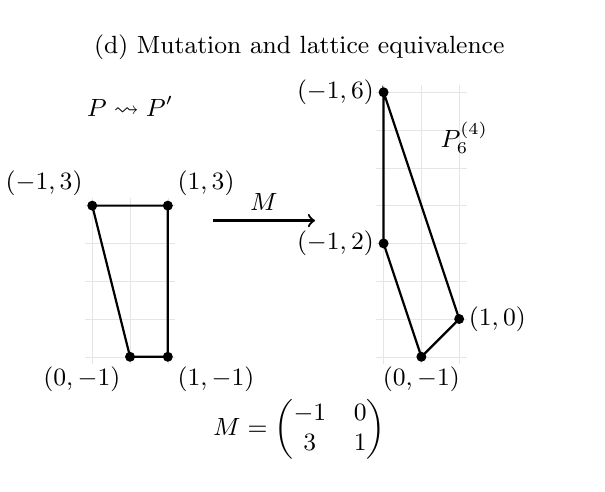
\begin{tikzpicture}[x=1cm,y=1cm,font=\small]
  \useasboundingbox (-1.3,-1.44) rectangle (5.68,4.1);
  \node at (2.15,3.85) {(d) Mutation and lattice equivalence};
  \node at (0,3.1) {$P\rightsquigarrow P'$};
  \begin{scope}[x=0.48cm,y=0.48cm,yshift=0.4cm]
    \draw[step=1,gray!20,very thin] (-1.2,-1.2) grid (1.2,3.2);
    \draw[thick] (-1,3)--(1,3)--(1,-1)--(0,-1)--cycle;
    \foreach \horizontal/\vertical in {-1/3,1/3,1/-1,0/-1}
      \fill (\horizontal,\vertical) circle (1.8pt);
    \node[above left] at (-1,3) {$(-1,3)$};
    \node[above right] at (1,3) {$(1,3)$};
    \node[below right] at (1,-1) {$(1,-1)$};
    \node[below left] at (0,-1) {$(0,-1)$};
  \end{scope}
  \draw[->,thick] (1.05,1.65)--(2.35,1.65) node[midway,above] {$M$};
  \begin{scope}[x=0.48cm,y=0.48cm,xshift=3.7cm,yshift=0.4cm]
    \draw[step=1,gray!20,very thin] (-1.2,-1.2) grid (1.2,6.2);
    \draw[thick] (1,0)--(0,-1)--(-1,2)--(-1,6)--cycle;
    \foreach \horizontal/\vertical in {1/0,0/-1,-1/2,-1/6}
      \fill (\horizontal,\vertical) circle (1.8pt);
    \node[right] at (1,0) {$(1,0)$};
    \node[below] at (0,-1) {$(0,-1)$};
    \node[left] at (-1,2) {$(-1,2)$};
    \node[left] at (-1,6) {$(-1,6)$};
    \node[right] at (0.25,4.8) {$P_6^{(4)}$};
  \end{scope}
  \node at (2.15,-1) {$M=\begin{pmatrix}-1&0\\3&1\end{pmatrix}$};
\end{tikzpicture}
\end{minipage}

\smallskip
{\small
\[
\boxed{(g_{\mathrm{cat}},g_{\mathrm{cat}}^{\mathrm{qG}},g_{\mathrm{MMLP}})=(6,3,3)},
\qquad 6\xrightarrow[\delta=3]{T\text{-content}}3=3.
\]
}
\caption{The mixed-cone example of Example~\ref{ex:mixed-cone-delta}.  The top edge has width $5=3+2$ and height $3$, with an orange width-$3$ $T$-part and blue residual width $2$.  Two crepant subdivisions give different residual sets, each with two interior residual points.  After mutation the polygon is $\mathrm{GL}(2,\Z)$-equivalent to $P_6^{(4)}$.  The corresponding genera are $(6,3,3)$.}
\label{fig:mixed-cone-example}
\end{figure}

In this order its edges have absolute determinants $15,4,1$, widths $5,4,1$, and heights $3,1,1$.  The corresponding cones have types $\frac1{15}(1,4)$, $\frac14(1,3)=A_3$, and smooth, respectively.  The top edge has $w=\gcd(15,5)=5$ and $5=1\cdot3+2$; since $(4+1)/5=1$, its residue is $\frac16(1,1)$.  The $A_3$ cone has $m=4$, $w_0=0$, $\ell=1$, so contributes neither genus nor genus drop.

The interior lattice points are
\[
P^\circ\cap N=\{(0,0),(0,1),(0,2),(1,1),(1,2),(2,2)\}.
\]
The categorical and residual formulas give
\[
g_{\mathrm{cat}}(\mathcal X_P)=1+\frac{15-5}{2}=6,
\qquad
g_{\mathrm{cat}}^{\mathrm{qG}}(X_P)=1+\frac{2(3-1)}2=3,
\]
with drop $\binom32=3$.  The primitive generators on the top edge are $(-1,3),(1,3),(2,3),(4,3)$.  Cutting off its width-$3$ $T$-part at $(2,3)$ or at $(1,3)$ gives, respectively, residual triangles
\[
\begin{aligned}
\operatorname{conv}\{0,(2,3),(4,3)\},&\quad R\cap P^\circ=\{(1,1),(2,2)\},\\
\operatorname{conv}\{0,(-1,3),(1,3)\},&\quad R\cap P^\circ=\{(0,1),(0,2)\}.
\end{aligned}
\]
Thus Definition~\ref{def:residual-lattice-points} gives genuinely different residual sets, but their interior cardinality is $2$ in either subdivision.

Mutation with weight $(0,-1)$ and factor $[0,(1,0)]$ gives
\[
P'=\operatorname{conv}\{(-1,3),(1,3),(1,-1),(0,-1)\}.
\]
The unimodular matrix $\left(\begin{smallmatrix}-1&0\\3&1\end{smallmatrix}\right)$ maps its vertex set to $\{(1,0),(0,-1),(-1,2),(-1,6)\}$.  This is precisely Cavey--Prince's $P_6^{(4)}$ \cite[Section 4.1]{CP}.  Their Proposition~4.2 constructs a general deformation in the family $X_6^{(4)}$, the blow-up of $\Pj(1,1,6)$ at four general smooth points \cite[Definition 2.7]{CP}; mutation preserves the generic $\Q$-Gorenstein deformation class \cite[Theorem 3]{ACC+}.  The dual polygon has vertices $(0,-1/3),(-1,1),(4,1)$, so
\[
K_{X_P}^2=2\operatorname{Area}(P^\vee)=\frac{20}{3}
=6-4+4+\frac46,
\]
agreeing with the cascade degree $(k+2)^2/k-l$ \cite[Remark 2.8]{CP}.  The sole remaining singularity is $\frac16(1,1)$; applying Theorem~\ref{thm:cyclic-rank} to the canonical stack of $X_6^{(4)}$ gives $g_{\mathrm{cat}}=1+2=3$.

An explicit normalized maximally mutable Laurent polynomial for $P$ is
\[
\boxed{\begin{aligned}
f={}&x^{-1}y^3(1+x)^3(1+cx+x^2)\\
&+(1+x)^2(a+4x)y^2+(1+x)(b+6x)y+4x+y^{-1}.
\end{aligned}}
\]
Here the top factor $(1+x)^3$ represents the $T$-part, and $1+cx+x^2$ is the residual quadratic.  The $y^2$- and $y$-slices have the required factors $(1+x)^2$ and $1+x$.  Along the right edge, the coefficients $1,4,6,4,1$ give $y^{-1}(1+xy)^4$; the remaining edge is primitive.  These are exactly the conditions of \cite[Propositions 3.7 and 3.9]{CKPT}.  All exponents lie in $P$, the three vertex coefficients are $1$, and the constant coefficient is $0$.  The independent coefficients at the residual points $(0,1),(0,2),(0,3)$ of the second subdivision are $b,a,c+3$, respectively.  We obtain this polynomial from the divisibility conditions.

Let $\overline C_\eta$ be the toric closure of $f=\eta$.  It has arithmetic genus $6$.  Its Newton triangle is Minkowski indecomposable: any nontrivial lattice summands of a triangle would be homothetic triangles, whereas its edge lengths $5,4,1$ have greatest common divisor $1$.  A nontrivial factorization would induce such a decomposition, so the curve is irreducible.  Its torus part is smooth for general $\eta$.

At the right boundary use $s=xy$ and $z=y$, with boundary $z=0$.  The local equation $z(f-\eta)=0$ restricts to $(1+s)^4$, and its transverse derivative at $(s,z)=(-1,0)$ is $a-b-c-\eta-1$.  For general parameters the point is smooth, with order-$4$ tangency and $\delta=0$.  At the top boundary put $t=x+1$, $u=y^{-1}$.  The equation $xu^3(f-\eta)=0$ has no terms of total degree below $3$, and its cubic part is
\[
\boxed{(2-c)t^3+(4-a)t^2u+(6-b)tu^2+(4+\eta)u^3.}
\]
This binary cubic has distinct roots for general parameters: at $a=b=c=\eta=0$ its discriminant is $-448$.  The point is therefore an ordinary triple point with $\delta=3$.  For general $c$, the residual quadratic has two simple roots different from $-1$, giving transverse intersections with the top boundary.  The primitive third edge also gives a transverse intersection, and there are no further boundary singularities.  Consequently
\[
g\bigl(\widetilde{\overline C_\eta}\bigr)=6-3=3,
\qquad
\boxed{(g_{\mathrm{cat}},g_{\mathrm{cat}}^{\mathrm{qG}},g_{\mathrm{MMLP}})=(6,3,3).}
\]
The ordinary triple point realizes $\delta=1\binom32=3$ in Proposition~\ref{prop:boundary-delta}, exactly the contribution of the width-$3$, height-$3$ $T$-part of this mixed cone.
\end{example}

\begin{example}[The five-point surface $X_{5,5/3}$]\label{ex:five-point-toric}
Corti--Heuberger give a toric $\Q$-Gorenstein degeneration of $X_{5,5/3}$ with polygon $P_7$ \cite[Section 7 and Table 4, polygon 7]{CH}:
\[
P_7=\operatorname{conv}\{(2,1),(1,2),(-1,2),(-2,1),(-2,-1),(-1,-2),(1,-1)\}.
\]
The edge cones consist of five $\frac13(1,1)$ points with $(w,\ell)=(1,3)$ and two $\frac14(1,1)$ points with $(w,\ell)=(2,2)$.  Thus
\[
g_{\mathrm{cat}}(\mathcal X_{P_7})=1+5\cdot1+2\cdot1=8.
\]
The two $T$-singularities each contribute a drop of $\binom22=1$ under smoothing, while the five residual points persist.  Corollaries~\ref{cor:t-content-drop} and~\ref{cor:qg-generic-mirror-genus} give
\[
g_{\mathrm{cat}}^{\mathrm{qG}}(X_{P_7})=8-2=6,
\qquad \boxed{g_{\mathrm{MMLP}}=6=5+1.}
\]
This closes the apparent $k=5$ gap in the Oneto--Petracci calculations discussed above using the toric degeneration, independently of the uncomputed Oneto--Petracci quantum period.
\end{example}

\begin{example}[The $X_{10}$ mirror polygon: a drop of $34$]\label{ex:x10-toric-drop}
Return to the triangle $P$ in Example~\ref{ex:x10-mirror-polygon}, and let $X_P$ be the toric surface defined by the fan over its edges, with canonical stack $\mathcal X_P$.  Its three edge cones have width--height pairs
\[
(w,\ell)=(10,3),\quad(10,5),\quad(10,2).
\]
Theorem~\ref{thm:cyclic-rank} and Proposition~\ref{prop:toric-categorical-genus} give
\[
g_{\mathrm{cat}}(\mathcal X_P)=1+10+20+5=36=\#(P^\circ\cap\Z^2).
\]
The width decompositions are $10=3\cdot3+1$, $10=2\cdot5$, and $10=5\cdot2$, so the only residue has width one and height three, of type $\frac13(1,1)$.  Consequently Proposition~\ref{prop:qg-residual-genus} and Corollary~\ref{cor:t-content-drop} give
\[
g_{\mathrm{cat}}^{\mathrm{qG}}(X_P)=2,\qquad
36-2=\frac12\bigl(3\cdot3\cdot2+2\cdot5\cdot4+5\cdot2\cdot1\bigr)=34.
\]
Figure~\ref{fig:x10-subdivision} displays these $34$ discarded points.  The genus-two curve in \eqref{eq:x10-hyperelliptic} realizes this residual genus explicitly.  It is the canonical stack of the toric degeneration that has genus $36$, not $\cX_{10}$, whose categorical genus is already two.
\end{example}

For a toric surface $X_P$ and a sufficiently general $\Q$-Gorenstein deformation $X_t$, the comparison is summarized by
\[
\begin{array}{c|c|c}
g_{\mathrm{cat}}(\mathcal X_P)&g_{\mathrm{cat}}(\mathcal X_t)&g_{\mathrm{MMLP}}\\\hline
\#(P^\circ\cap N)&1+\#(R\cap P^\circ)&1+\#(R\cap P^\circ)
\end{array}
\]
The first column is also the genus of a general nondegenerate Laurent-polynomial fiber with polygon $P$; the last column uses a general maximally mutable Laurent polynomial with the specified Newton polygon.  The difference between them is the weighted $T$-content contribution in Corollary~\ref{cor:t-content-drop}.  Petracci's example gives $(9,7,7)$ with separate rigid and pure $T$-cones.  Example~\ref{ex:mixed-cone-delta} gives $(6,3,3)$ from a genuinely mixed cone with $m>0$ and $w_0=2$.  Example~\ref{ex:five-point-toric} gives $(8,6,6)$, closing the $k=5$ gap, while Example~\ref{ex:x10-toric-drop} gives $(36,2,2)$ and a much larger $T$-content drop.

\begin{remark}[The scope of the mirror comparison]\label{rem:johnson-kollar-mirror}
Theorem~\ref{thm:intro-mirror} and Corollary~\ref{cor:qg-generic-mirror-genus} concern maximally mutable Laurent polynomial mirrors associated with toric $\Q$-Gorenstein degenerations.  The Johnson--Koll\'ar surfaces of Example~\ref{ex:johnson-kollar-categorical} have empty anticanonical system and therefore admit no such degeneration \cite[Section 1.1]{GR}.  Corti--Gugiatti construct hyperelliptic Landau--Ginzburg mirrors in the sense of matching periods, with general fiber of genus $3k+1$ \cite[Remarks 1.4 and 1.7 and Theorem 1.5]{CG}, whereas $g_{\mathrm{cat}}=6k+1$.  In this family the numerical values satisfy $2g_{\mathrm{mirror}}=g_{\mathrm{cat}}+1$; Theorem~\ref{thm:intro-mirror} does not apply because the surfaces admit no toric $\Q$-Gorenstein degeneration.
\end{remark}

\appendix
\section{The numerical inertial decomposition}\label{app:numerical-inertia}

Proposition~\ref{prop:numerical-inertia} requires an identification of numerical $K$-theory with numerical Chow theory of the inertia stack.  We prove this identification first, then use the isolated cyclic quotient geometry to separate one untwisted component from one twisted component for every nonidentity stabilizer element.  Throughout, $X$ is a projective surface with isolated cyclic quotient singularities $\frac1{n_j}(1,q_j)$, and $\cX$ is its canonical stack.

\begin{definition}[Grothendieck group]
Throughout the paper we use the convention
\[
K_0(\cX)=K_0\bigl(\Db(\coh\cX)\bigr)=G_0(\cX),
\]
where the last identification is induced by the alternating sum of coherent cohomology sheaves.
\end{definition}

Thus the Riemann--Roch theorem on $G_0$ applies to our $K_0$; no identification with vector-bundle $K$-theory is required.  Pullbacks, tensor products, and duals of coherent complexes below are derived.  Since $\cX$ is smooth, bounded coherent complexes are perfect, so the derived tensor product and derived dual used below remain in $\Db(\coh\cX)$.

The connected components of $I\cX$ are smooth in characteristic zero.  On a component $F$ of dimension $d$, cap product with $[F]$ identifies $A^p(F)$ with $A_{d-p}(F)$; we therefore write the Chow-homological Riemann--Roch maps in cohomological notation $A^*$.  Complexification separates the finite stabilizer representations into character eigenspaces and does not change the ranks used in Section~\ref{sec:serre}.

Working over $\C$ does not change the numerical quotient: for $V=K_0(\cX)_{\Q}$,
\[
\operatorname{rad}(\chi_{\C})=(\operatorname{rad}\chi_{\Q})\otimes_{\Q}\C.
\]
Indeed, write a complexified class as a finite sum with $\Q$-linearly independent complex coefficients.  If its Euler pairing with every rational class vanishes, each rational coefficient class is in the radical.  Thus extension of scalars commutes with passing to numerical equivalence.

The argument passes through the following maps, whose numerical compatibility and sector decomposition will be justified separately:
\[
\begin{aligned}
K_0(\cX)_{\C}&\xrightarrow{\ \widetilde{\operatorname{ch}}\ } A^*(I\cX)_{\C},\\
K_0^{\mathrm{num}}(\cX)_{\C}&\simeq A^*_{\mathrm{num}}(I\cX)_{\C},\\
A^*_{\mathrm{num}}(I\cX)_{\C}&\simeq A^*_{\mathrm{num}}(\cX)_{\C}
\oplus\bigoplus_j\bigoplus_{i=1}^{n_j-1}\C_{j,i}.
\end{aligned}
\]

\begin{definition}[Inertia morphism]
Recall that the inertia stack $I\cX$ parametrizes pairs $(x,g)$, where $g$ is an automorphism of $x$.  The identity automorphism gives the \emph{untwisted sector}, isomorphic to $\cX$; the connected components with $g\ne1$ are the \emph{twisted sectors}.  The inertia map $e:I\cX\to\cX$ forgets the automorphism.
\end{definition}

We use the inertial Chern character of \eqref{eq:inertial-character-convention}: each eigenbundle contributes its ordinary Chern character weighted by the eigenvalue of the sector element.  This is Edidin's eigenvalue-twisting construction \cite[Section 4.3.2]{Edidin}; it is multiplicative and extends linearly to $K_0(\cX)_{\C}$.

\begin{definition}[Numerical Chow groups]
For a smooth proper stack $Z$, possibly disconnected, write $A^*_{\mathrm{num}}(Z)_{\C}$ for its Chow group modulo the radical of the intersection pairing $\langle\alpha,\beta\rangle=\int_Z\alpha\beta$.  Integration sums the degrees of the zero-dimensional parts over the connected components.  In particular, $\alpha$ is numerically trivial precisely when this integral vanishes for every $\beta$.
\end{definition}

On the untwisted component we use the ordinary intersection product on the smooth stack $\cX$.  The comparison with the coarse surface is made afterwards via Vistoli's rational coarse-space correspondence, in Lemma~\ref{lem:untwisted-rank}.

The first two lemmas record the standard Riemann--Roch machinery: the inertial Chern character is an isomorphism, and its expression for the Euler pairing identifies the numerical radicals.  The next two lemmas specialize to the cyclic quotient geometry, describing the inertia components and their numerical Chow groups.  A final lemma checks compatibility with tensoring by the canonical bundle, which is the feature needed for the Serre calculation in Section~\ref{sec:serre}.

\begin{lemma}[Inertial Chern character and Riemann--Roch]\label{lem:app-inertial-ch}
Let $N_e=(e^*T_{\cX})^{\mathrm{mov}}$ be the normal bundle of the inertia map, and let $t$ denote Edidin's eigenvalue-twisting operator from \cite[Section 4.3.2]{Edidin}, with the convention of \eqref{eq:inertial-character-convention}.  The inertial Riemann--Roch isomorphism $\tau={}^I\tau_{\cX}$ of \cite[Theorem 5.1]{Edidin} has the form
\[
\tau(v)=\widetilde{\operatorname{ch}}(v)\,\mathcal T,
\qquad
\mathcal T|_F=
\frac{\operatorname{td}(T_F)}
{\operatorname{ch}\bigl(t(\lambda_{-1}(N_e^\vee|_F))\bigr)}
\]
on each component $F\subset I\cX$, where $\lambda_{-1}(N_e^\vee)=\sum_a(-1)^a[\bigwedge^aN_e^\vee]$.  The class $\mathcal T$ is a unit in $A^*(I\cX)_{\C}$.  Consequently
\[
\widetilde{\operatorname{ch}}:K_0(\cX)_{\C}\xrightarrow{\sim}A^*(I\cX)_{\C}
\]
is an isomorphism of complex vector spaces.
\end{lemma}

\begin{proof}
The quotient-stack theorem applies: stabilizers act faithfully on $T_{\cX}$, so its frame bundle is an algebraic space presenting $\cX$ as a quotient by $\operatorname{GL}_2$.  Edidin \cite[Theorem 5.1]{Edidin} supplies the isomorphism on $G_0$ with formula
\[
\tau(v)=\operatorname{ch}\!\left(t\!\left(
\frac{e^*v}{\lambda_{-1}(N_e^\vee)}\right)\right)
\operatorname{td}(T_{I\cX}).
\]
Here $e$ and $N_e^\vee$ are his $f$ and $N_f^*$; multiplicativity and $\widetilde{\operatorname{ch}}(v)=\operatorname{ch}(t(e^*v))$ give the stated factorization.  Krishna--Sreedhar \cite[Theorem 1.2]{KrishnaSreedhar} provide the more general Atiyah--Segal/Riemann--Roch framework.

On the untwisted component, $N_e=0$ and $\mathcal T=\operatorname{td}(T_{\cX})$ has constant term $1$.  On a twisted component, every moving eigenvalue differs from $1$, so the denominator has nonzero constant term; the Todd numerator has constant term $1$.  Thus $\mathcal T$ has nonzero degree-zero term on every component.  Positive-codimension classes are nilpotent, so $\mathcal T$ is a unit.  Multiplication by $\mathcal T^{-1}$ turns $\tau$ into the asserted Chern-character isomorphism.
\end{proof}

To pass to numerical equivalence, we must express dualization in these coordinates.

\begin{definition}[Duality on the inertia Chow group]
Let $\iota:I\cX\to I\cX$ send $(x,g)$ to $(x,g^{-1})$.  This is an involutive automorphism of the inertia stack, so $\iota^*$ is an isomorphism of its Chow groups.  For $\alpha=\sum_p\alpha_p$, with $\alpha_p\in A^p(I\cX)_{\C}$, define
\[
\alpha^\dagger=\iota^*\left(\sum_p(-1)^p\alpha_p\right).
\]
\end{definition}
Dualization reverses the character eigenvalues and multiplies the codimension-$p$ Chern character by $(-1)^p$.  Hence this $\C$-linear involution, which is not complex conjugation, encodes duality as
\[
\widetilde{\operatorname{ch}}(v^\vee)=\widetilde{\operatorname{ch}}(v)^\dagger.
\]

\begin{lemma}[Compatibility with numerical equivalence]\label{lem:app-numerical}
The inertial Chern character induces an isomorphism
\[
K_0^{\mathrm{num}}(\cX)_{\C}\simeq A^*_{\mathrm{num}}(I\cX)_{\C}.
\]
\end{lemma}

\begin{proof}
Let $p:\cX\to\operatorname{Spec}\C$ be the structure morphism and put
\[
a=v^\vee\otimes^{\mathbf L}w.
\]
By the proper-pushforward compatibility of inertial Riemann--Roch on $G_0$ for $p$ \cite[Theorem 5.1 and Corollary 5.3]{Edidin},
\[
\chi(v,w)=\int_{I\cX}{}^I\tau_{\cX}(a).
\]
Using Lemma~\ref{lem:app-inertial-ch}, multiplicativity of the inertial Chern character, and the duality convention above, this becomes
\begin{equation}\label{eq:inertial-euler-pairing}
\chi(v,w)=\int_{I\cX}
\widetilde{\operatorname{ch}}(v)^\dagger
\widetilde{\operatorname{ch}}(w)\,\mathcal T.
\end{equation}
Write $A=A^*(I\cX)_{\C}$ and let $N$ be the radical of its intersection pairing.  We check explicitly that the two operations modifying that pairing in \eqref{eq:inertial-euler-pairing} preserve $N$.

First, $N$ is an ideal: if $\alpha\in N$ and $u,\beta\in A$, then $\int\alpha u\beta=0$, since $u\beta$ is another test class.  Multiplication by $\mathcal T$ therefore preserves $N$, and so does multiplication by $\mathcal T^{-1}$.  Thus $\alpha\mathcal T\in N$ if and only if $\alpha\in N$.

Second, $N$ is graded, because classes of each codimension can be tested against complementary codimensions on each component.  Changing the codimension-$p$ part by $(-1)^p$ therefore preserves $N$.  The isomorphism $\iota$ permutes the components and preserves intersection degrees, so $\iota^*$ also preserves $N$.  Since $\dagger$ is an involution, $\alpha^\dagger\in N$ if and only if $\alpha\in N$.

Finally, put $\alpha=\widetilde{\operatorname{ch}}(v)$.  By Lemma~\ref{lem:app-inertial-ch}, the classes $\widetilde{\operatorname{ch}}(w)$ run through all of $A$.  Multiplication by the unit $\mathcal T$ leaves this set of test classes unchanged.  Consequently
\[
\begin{aligned}
\chi(v,w)=0\text{ for every }w
&\quad\Longleftrightarrow\quad
\int_{I\cX}\alpha^\dagger\beta=0\text{ for every }\beta\in A\\
&\quad\Longleftrightarrow\quad \alpha^\dagger\in N
\quad\Longleftrightarrow\quad \alpha\in N.
\end{aligned}
\]
Thus Euler-numerical triviality is exactly numerical triviality under the inertial Chern character.  Quotienting the isomorphism of Lemma~\ref{lem:app-inertial-ch} by these corresponding radicals proves the result.
\end{proof}

The Riemann--Roch step is complete.  We now use the specific geometry of isolated cyclic quotient points to identify the numerical summands.

\begin{lemma}[Twisted sectors of isolated cyclic quotient points]\label{lem:app-sectors}
The inertia stack of $\cX$ decomposes as
\[
I\cX=\cX\sqcup\coprod_j\coprod_{i=1}^{n_j-1}\mathcal B\mu_{n_j}^{(i)}.
\]
\end{lemma}

\begin{proof}
The canonical stack has trivial stabilizers away from the singular points.  Near a point of type $\frac1n(1,q)$, a nonidentity element $\zeta^i\in\mu_n$ has tangent eigenvalues $\zeta^i$ and $\zeta^{iq}$.  Both differ from $1$ because $1\le i\le n-1$ and $\gcd(n,q)=1$, so its fixed locus is the origin.  Since $\mu_n$ is abelian, each nonidentity element gives one inertia component $[\{0\}/\mu_n]=\mathcal B\mu_n$.  Together with the identity sector, these are all the components.
\end{proof}

\begin{lemma}[Numerical Chow groups of twisted gerbes]\label{lem:app-gerbe-chow}
For a twisted component $\mathcal B\mu_n$,
\[
A^*_{\mathrm{num}}(\mathcal B\mu_n)_{\C}\simeq\C,
\]
concentrated in codimension zero.
\end{lemma}

\begin{proof}
The rational coarse-space correspondence \cite[Proposition 6.1]{Vistoli} identifies the Chow groups of $\mathcal B\mu_n$ with those of a point.  Thus $A^*(\mathcal B\mu_n)_{\C}$ is one-dimensional in codimension zero, with no positive-codimension part.  Its fundamental class has degree $\deg[\mathcal B\mu_n]=1/n\ne0$ \cite[Section 3.2.1]{Edidin}, so it survives numerical equivalence.
\end{proof}

It remains to check that the sector decomposition is preserved by the Serre operator.

\begin{lemma}[Compatibility with the Serre operator]\label{lem:app-serre}
Under the inertial Chern character, tensor product with a line bundle $L$ acts by multiplication by $\widetilde{\operatorname{ch}}(L)$.  In particular, the Serre operator $S_{\cX}$ preserves every summand of the numerical inertial decomposition.
\end{lemma}

\begin{proof}
By the ideal property of the numerical radical established in Lemma~\ref{lem:app-numerical}, multiplication by $\widetilde{\operatorname{ch}}(L)$ preserves that radical and therefore descends to $A^*_{\mathrm{num}}(I\cX)_{\C}$.  Multiplicativity gives
\[
\widetilde{\operatorname{ch}}(v\otimes L)
=\widetilde{\operatorname{ch}}(v)\,\widetilde{\operatorname{ch}}(L).
\]
Products on the Chow ring of the disjoint union $I\cX$ are componentwise, so every inertia-sector summand is preserved.  On a surface stack the Serre functor is tensor product with $\omega_{\cX}[2]$; the shift acts trivially on $K_0$.  Taking $L=\omega_{\cX}$ proves the assertion.  Thus the rank of $1-S_{\cX}$ can be computed separately on each summand, as used in Section~\ref{sec:serre}.
\end{proof}

\begin{proof}[Proof of Proposition~\ref{prop:numerical-inertia}]
Lemma~\ref{lem:app-numerical} gives $K_0^{\mathrm{num}}(\cX)_{\C}\simeq A^*_{\mathrm{num}}(I\cX)_{\C}$.  Lemma~\ref{lem:app-sectors} decomposes the inertia into $\cX$ and the components $\mathcal B\mu_{n_j}^{(i)}$, whose numerical Chow groups are each $\C$ by Lemma~\ref{lem:app-gerbe-chow}.  Since the intersection pairing is componentwise, these identifications yield
\[
\boxed{
K_0^{\mathrm{num}}(\cX)_{\C}
\overset{\widetilde{\operatorname{ch}}}{\simeq}
A^*_{\mathrm{num}}(I\cX)_{\C}
\simeq A^*_{\mathrm{num}}(\cX)_{\C}
\oplus\bigoplus_j\bigoplus_{i=1}^{n_j-1}\C_{j,i}.}
\]
Lemma~\ref{lem:app-serre} makes this decomposition $S_{\cX}$-invariant.  This proves the intrinsic assertion about the stack; Vistoli's comparison with $X$ is used only afterwards, in the untwisted calculation of Lemma~\ref{lem:untwisted-rank}.
\end{proof}

\section*{Acknowledgements}

The author thanks Sergey Galkin for pointing out the genus-two phenomenon for the mirror of $X_{10}$ and suggesting its relation to the antisymmetric Euler pairing.  The author also thanks Sergei Burkin for teaching him the modern viewpoint on characteristic classes, which influenced the Chern-character and Riemann--Roch perspective used here.

\section*{Funding}

% Funding follows the author's reference manuscript; confirm applicability before submission.
The author acknowledges support from FAPERJ (Funda\c{c}\~ao Carlos Chagas Filho de Amparo \`a Pesquisa do Estado do Rio de Janeiro) through its Nota~10 Excellence Scholarship.

\section*{Declaration of generative AI and AI-assisted technologies in the writing process}

During the preparation of this manuscript, the author used ChatGPT (OpenAI) for language editing, organization, \LaTeX{} formatting, bibliographic research, mathematical exposition, and exploratory symbolic and numerical checks.  The author independently checked all mathematical statements, proofs, computations, and uses of references, and takes full responsibility for the final manuscript.

\printbibliography

\end{document}